% This must be in the first 5 lines to tell arXiv to use pdfLaTeX, which is strongly recommended.
\pdfoutput=1
% In particular, the hyperref package requires pdfLaTeX in order to break URLs across lines.

\documentclass[11pt]{article}

% Remove the "review" option to generate the final version.
\usepackage[review]{ACL2023}

% ACL2023.sty hardcodes margin=2.5cm on every side; narrow the side margins here
% (rather than editing the vendor style file) to widen the text column and the
% abstract/title block, which spans the same width via \twocolumn[...].
\geometry{left=1.8cm,right=1.8cm}

% Standard package includes
\usepackage{times}
\usepackage{latexsym}
\usepackage{amsmath,amssymb}
\usepackage[capitalize]{cleveref}

% For proper rendering and hyphenation of words containing Latin characters (including in bib files)
\usepackage[T1]{fontenc}
% This assumes your files are encoded as UTF8
\usepackage[utf8]{inputenc}

% Improves layout / spacing
\usepackage{microtype}
\usepackage{inconsolata}

\usepackage{graphicx}
\usepackage{booktabs}
\usepackage{tikz}

% If the title and author information does not fit in the area allocated, uncomment the following
%\setlength\titlebox{<dim>}

\title{Auditing HeSum: Reference Quality Defects in a Hebrew News Summarization Corpus}

\author{
  Amit Benbenishti \\ \texttt{<email>} \And
  Avraham Asraf \\ \texttt{<email>} \And
  Ofek Varona \\ \texttt{<email>}
}

\begin{document}
\maketitle

\begin{abstract}
Hebrew news summarization is commonly trained on HeSum, a corpus of article--headline pairs scraped
from Hebrew news sites and used as-is for the training target. We argue that a large share of these
targets are unfit to train on, and that this, not model capacity, is the field's real bottleneck. The
evidence came from two fine-tuning attempts, neither originally designed as a data audit.
\texttt{Qwen3-2B}, fine-tuned on HeSum, learned the corpus's headline style without learning to be
faithful to the article it summarized. Switching to the Hebrew-native
\texttt{dicta-il/dictalm2.0-instruct} fixed fluency, but surfaced a harder problem: its zero-shot
summaries routinely read as \emph{better} than the references they were scored against. Both failures
pointed past the model and into the data, so we stopped fine-tuning and audited the corpus instead. We
built a multi-stage curation pipeline and a four-dimension rubric judge (faithfulness, single-focus,
informativeness, cleanliness) that reads the source article directly and scores a headline without
needing a second reference string to compare it against. A large share of the corpus fails this audit
outright, and most of what survives still needs its headline rewritten. Flagged rows score measurably
worse on every rubric dimension, and in a blind head-to-head comparison curated headlines are strongly
preferred over the originals---while a placebo comparison on untouched rows confirms the judge isn't
just guessing. We report this as a dataset review rather than a model-building exercise, and close with
the training comparison (curated vs.\ original headlines, identical articles) that was still in progress
at submission time.
\end{abstract}

\section{Introduction}

\paragraph{What we are trying to do.}
We check whether the headlines used to train Hebrew news summarizers are actually good enough to
learn from, and whether fixing the bad ones changes what a model learns. The dataset in question,
HeSum \citep{paz-argaman2024hesum}, is one of the few Hebrew resources large enough to fine-tune a
modern language model on, so if its targets are flawed, that flaw reaches further than one project.

\paragraph{How this is done today, and its limits.}
The usual recipe for a new-language summarization paper is to fine-tune an instruction model on the
available corpus, then report ROUGE, BERTScore \citep{zhang2020bertscore}, and an LLM judge scored
against the corpus's own references -- every step of which treats those references as correct. That
assumption does not hold automatically for a corpus scraped from news sites: HeSum's own documentation
describes its summaries as extended subheadings lifted from articles, not summaries written for the
task, and \citet{nallapati2016abstractive} and \citet{see2017get} already showed that references built
this way tend to be lead-aligned, rewarding a model for copying the opening sentence rather than
actually summarizing.

\paragraph{What is new here, and why we expect it to work.}
Instead of running one more fine-tuning attempt on an unaudited corpus, we flip the order: audit the
references first, train second. We built a multi-stage pipeline that removes or repairs the worst
headlines, and a rubric judge that reads the source article directly and scores a headline on four
independent dimensions, rather than comparing it to another string. Because the judge only needs the
article, it can score a human-written reference and a model's output on the identical scale, which is
what lets us connect the dataset audit directly to a training comparison. We pre-register the four
experiments this enables (Section~\ref{sec:methods}) so the paper's conclusions rest on effect sizes
decided in advance, not on hindsight.

\paragraph{Who this matters for.}
Anyone training a Hebrew summarizer on HeSum inherits whatever is wrong with it, whether they audit it
or not. If the problems are as common and as damaging as we find, the fix is not a bigger model -- it
is cleaning the targets before training starts. That is a claim about a public dataset that any future
HeSum user can act on, not just about the one model we happened to train.

\subsection{From a model question to a data question}
\label{sec:pivot}

The project began as a conventional fine-tuning study: fine-tune \texttt{Qwen/Qwen3-2B} on HeSum, compare
LoRA/QLoRA/full fine-tuning regimes, and probe whether the resulting model aggregates global context or
latches onto the article lead. Two findings redirected it.

\textbf{Era 1 -- Qwen3-2B.} Across three training iterations (Appendix~\ref{app:qwen}), suppressing a
repetition artifact that had been inflating ROUGE exposed a model that was fundamentally undertrained,
and once fixed, it produced fluent, correctly formatted Hebrew with \emph{wrong facts}: the LLM judge
rated the untuned base model as more faithful (2.98) than the fine-tuned one (2.64). A model that
reliably learns its targets' surface style without learning their content is usually telling you
something about the targets, not just the model.

\textbf{Era 2 -- DictaLM2.0.} Switching to a Hebrew-native base model
(\texttt{dicta-il/dictalm2.0-instruct}) produced an immediate qualitative jump -- fluent Hebrew, no
script leakage, no reasoning-block failures. But reading enough zero-shot outputs against their
references made an uncomfortable pattern hard to unsee: the model's headline was, often, \emph{better}
than the HeSum reference it was being scored against. That observation moved the investigation from the
model to the data.

\textbf{Era 3 -- this paper.} Reading the HeSum paper alongside the raw rows explained why. HeSum's
summaries are professional \emph{extended subheadings} scraped from news sites, not summaries purpose-
written for a modeling task, and that origin produces concrete defects: multi-headline digests bundled
into one target, roundups spanning several unrelated stories, and scraped boilerplate tails. The rest of
this paper is the audit, repair, and evaluation of that finding.

\subsection{Research questions}

\begin{description}
  \item[RQ1] Are the rows our deterministic filters and LLM labels flag as defective genuinely worse
  reference-quality, or is the flagging itself unreliable? (\textbf{E1})
  \item[RQ2] When a headline is rewritten during curation, is the rewrite an improvement, and by how
  much? (\textbf{E2}, graded; \textbf{E3}, forced-choice)
  \item[RQ3] Does a model trained on curated headlines produce measurably better outputs than one
  trained on the same articles with their original headlines? (\textbf{E4})
  \item[RQ4] How does reference quality and headline--lead overlap vary continuously with article
  length, independent of any single filter threshold?
\end{description}

RQ1, RQ2, and RQ4 are answered in this paper. RQ3 (E4) depends on an external fine-tuning run that was
still in flight at submission time; Section~\ref{sec:results} reports what is measured so far and the
exact form the missing comparison will take.

\subsection{Contributions}
\begin{enumerate}
  \item A multi-stage, reproducible curation pipeline for HeSum with a documented, sha256-pinned
  handoff between deterministic filtering and LLM labeling.
  \item A four-dimension reference-quality rubric judge, validated by test--retest agreement and a
  null-calibration placebo, reused unchanged to score both dataset references and model outputs.
  \item Pre-registered evidence that the flagged defects are real (E1) and that the repair helped
  (E2/E3), with effect sizes rather than significance carrying the conclusions.
  \item A training-comparison design (E4) that isolates the headline-repair effect from data-quantity
  and article-selection confounds, reported here with the skeleton in place and results pending.
\end{enumerate}

\section{Data}
\label{sec:data}

\subsection{Source corpus}
HeSum \citep{paz-argaman2024hesum} provides $10{,}000$ Hebrew news article--headline pairs
$\{\mathit{text}, \mathit{headline}\}$, scraped from news outlets. We treat the published headline as
the summarization target, matching how the corpus is used for headline-generation fine-tuning.

\subsection{Curation pipeline}
We built a multi-stage pipeline (Figure~\ref{fig:funnel}) that separates two independent deterministic
filters from a subsequent LLM labeling pass, so that filtering decisions do not depend on the model
that later labels the survivors:

\begin{enumerate}
  \item \textbf{Tail-boilerplate trimming.} $722$ rows had a repeated scraped tail (byline, related-links
  block) stripped from the article text.
  \item \textbf{Token-budget filter.} Rows where $\mathrm{tokens}(\mathit{text}) + \mathrm{tokens}
  (\mathit{headline}) > 4{,}000$ (DictaLM tokenizer) are removed: $2{,}659$ rows ($26.6\%$).
  \item \textbf{Multi-pipe headline filter.} Rows whose headline contains two or more \texttt{|}
  characters (three or more bundled segments) are removed: $2{,}412$ rows ($24.1\%$).
  \item \textbf{Intersection.} The two filters are independent and only combined here, leaving
  $6{,}486$ rows ($35.1\%$ removed before any model saw a row).
  \item \textbf{Source-usability labeling.} An LLM (\texttt{gpt-5.6-luna}) labels each of the $6{,}486$
  rows as usable or one of five unusable categories (Section~\ref{sec:taxonomy}): $5{,}854$ usable,
  $632$ unusable.
  \item \textbf{Headline curation.} The same model decides, for each of the $5{,}854$ usable rows,
  whether to keep the original headline or replace it: $2{,}785$ kept, $\mathbf{3{,}069}$
  \textbf{rewritten} ($52.4\%$ of survivors).
  \item \textbf{Final assembly.} $5{,}854$ records, a $41.5\%$ net reduction from the raw corpus.
\end{enumerate}

\begin{figure}[t]
  \centering
  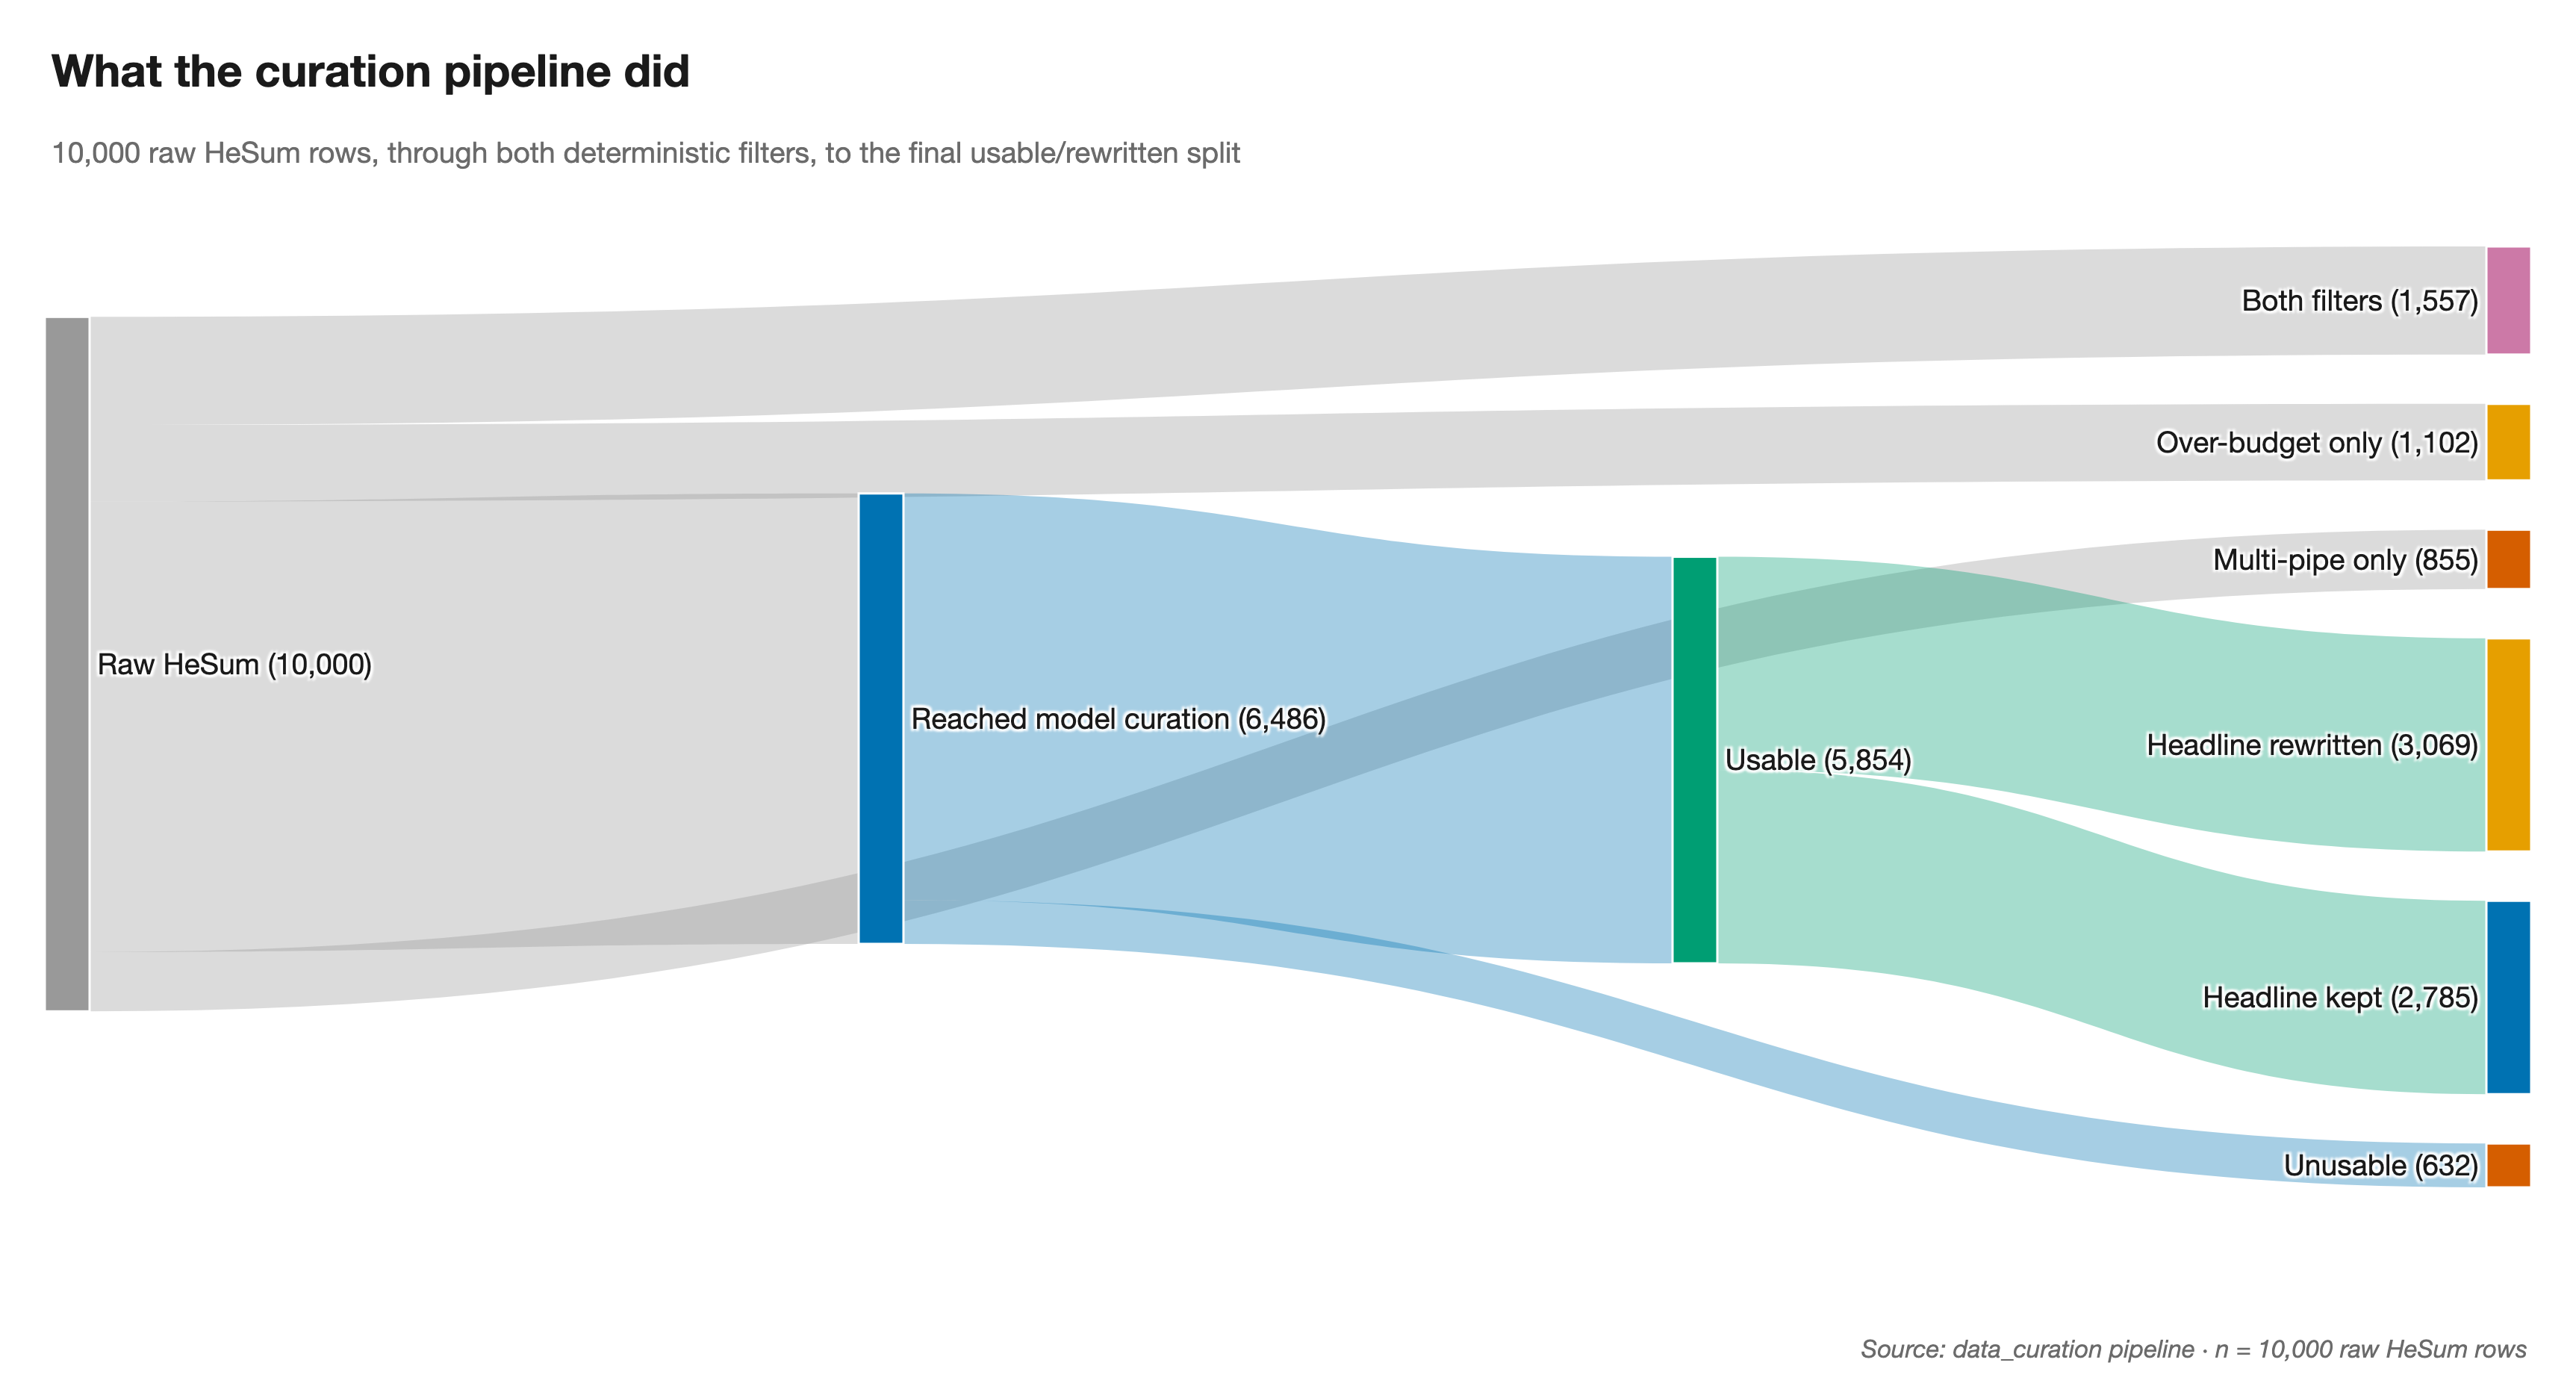
\includegraphics[width=\columnwidth]{figures/f1_curation_funnel.png}
  \caption{Curation funnel: the two independent deterministic filters converge before any row is
  labeled by a model, terminating in the kept-versus-rewritten headline fork.}
  \label{fig:funnel}
\end{figure}

\subsection{Defect taxonomy and analysis strata}
\label{sec:taxonomy}
The source-usability label defines six mutually exclusive categories with explicit negative guards; one
(\emph{other}) attracted zero rows across $6{,}486$ attempts, evidence the five substantive categories
are close to exhaustive on this corpus. We derive five \textbf{analysis strata} for the experiments in
Section~\ref{sec:methods}, overlapping by design since a row can carry more than one defect
(Table~\ref{tab:strata}, Figure~\ref{fig:prevalence}).

\begin{table}[t]
  \centering
  \small
  \begin{tabular}{lrl}
    \toprule
    \textbf{Stratum} & \textbf{$n$} & \textbf{Source} \\
    \midrule
    S0 clean & 2{,}785 & passed every filter \\
    S2 multi-pipe headline & 2{,}412 & deterministic ($\geq 2$ pipes) \\
    S3 multi-item & 569 & LLM label \\
    S4 headline rewritten & 3{,}069 & headline-curation decision \\
    S5 other unusable & 63 & LLM labels, collapsed \\
    \bottomrule
  \end{tabular}
  \caption{Analysis strata. S0 is the reference group for E1; S5 supports prevalence claims only (too
  small for a distributional test). Numbering skips S1 deliberately (see below).}
  \label{tab:strata}
\end{table}

\begin{figure}[t]
  \centering
  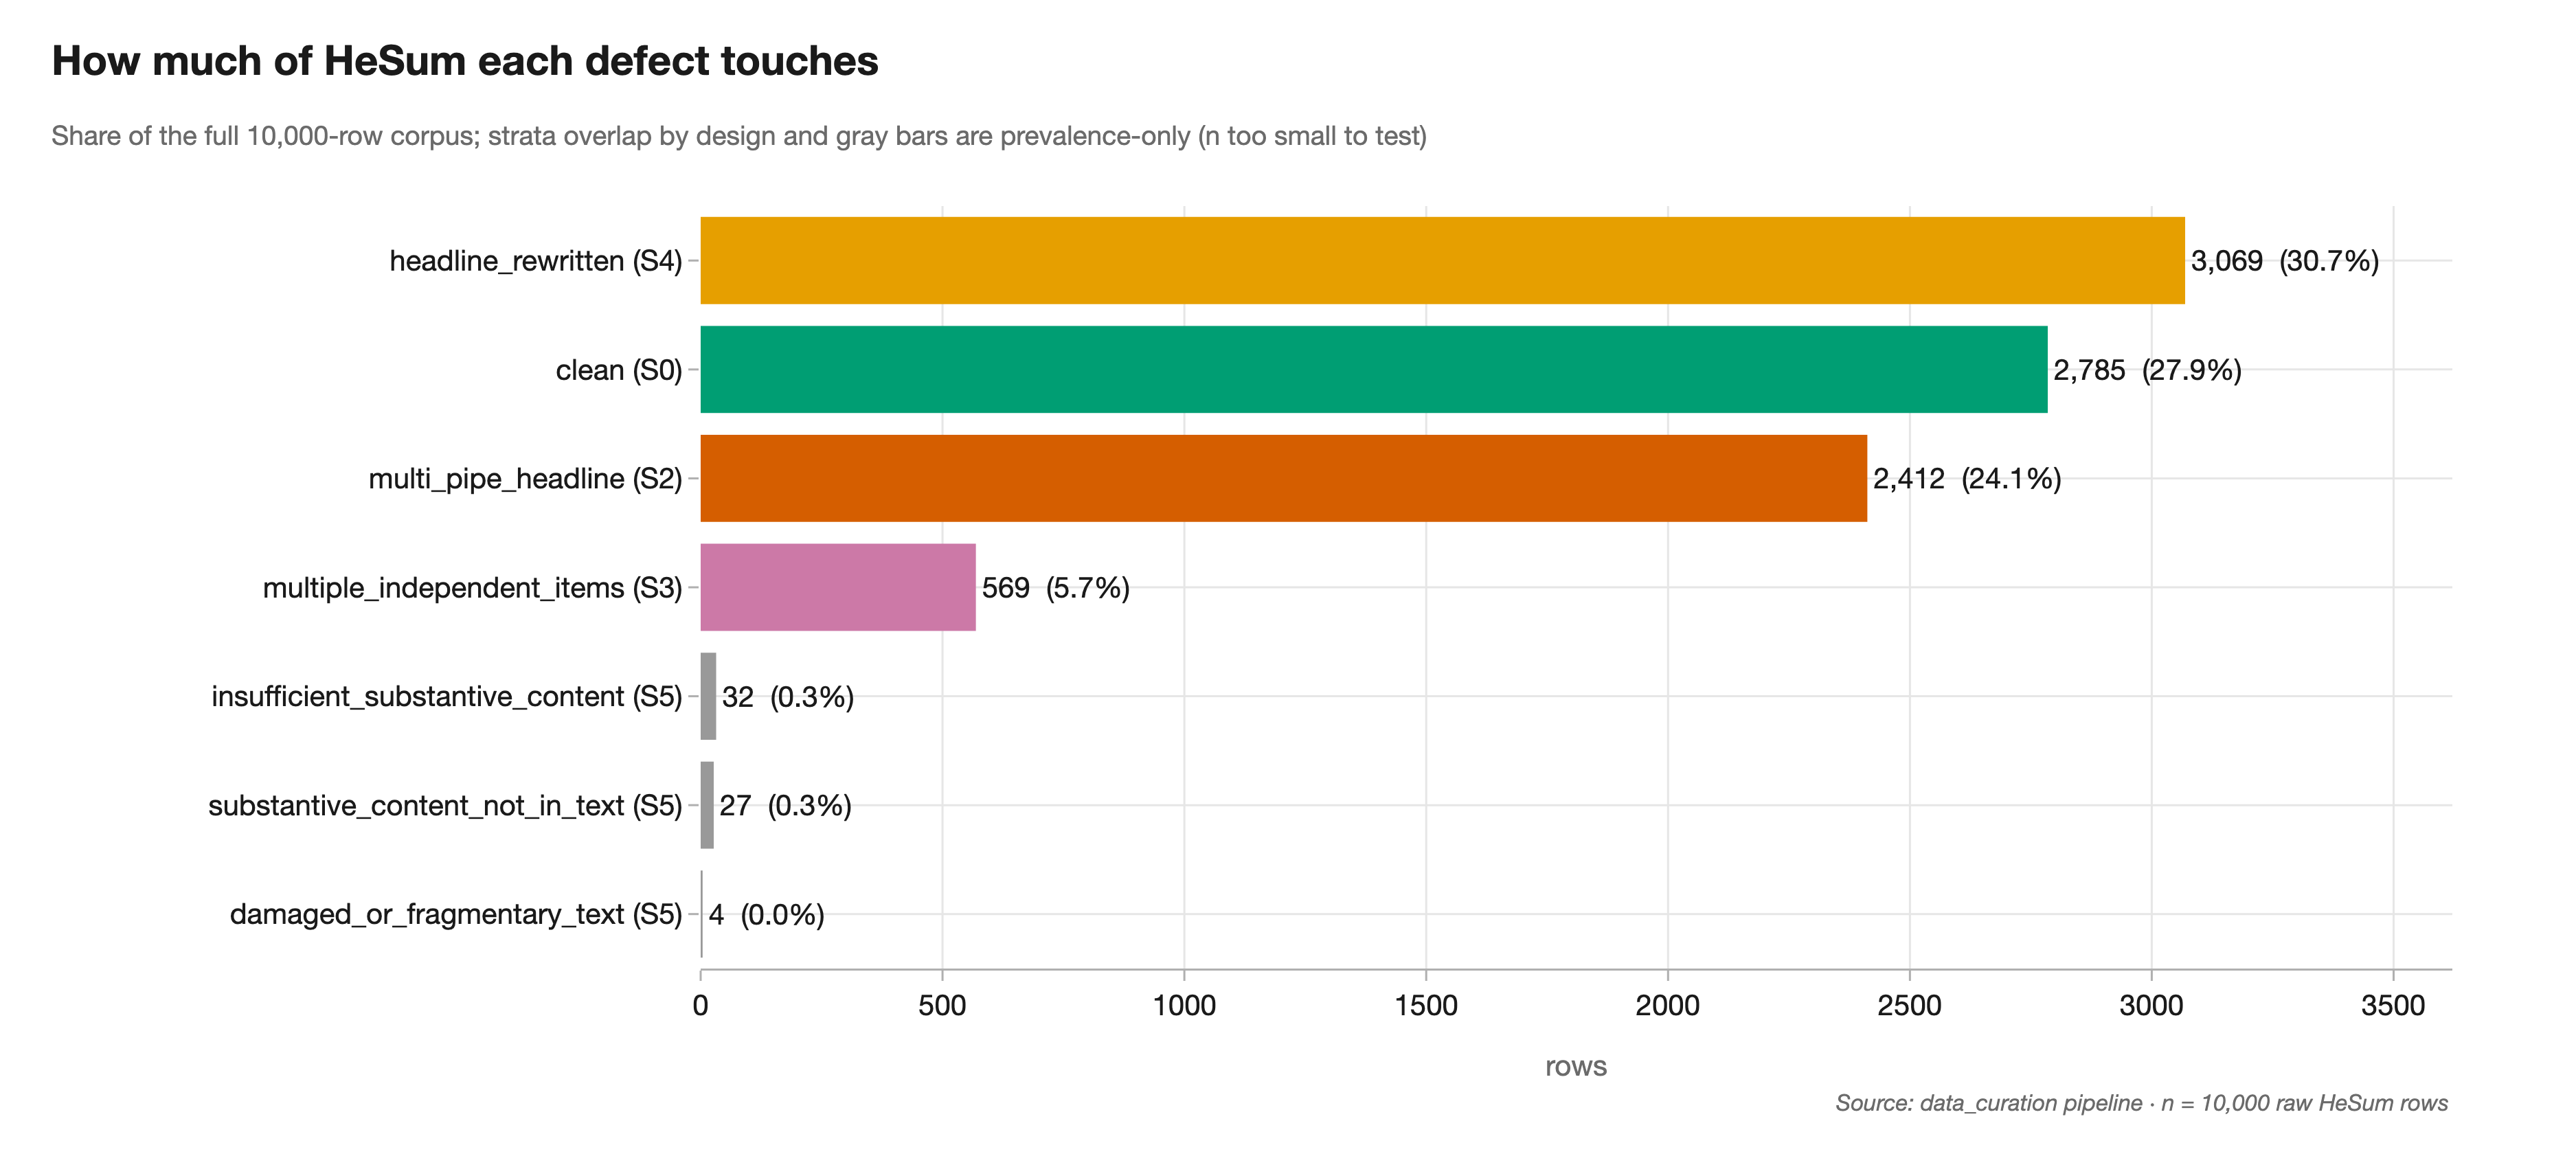
\includegraphics[width=\columnwidth]{figures/f2_defect_prevalence.png}
  \caption{Defect prevalence across the corpus, with \emph{other unusable} broken into its three
  constituent labels.}
  \label{fig:prevalence}
\end{figure}

\paragraph{Why article length is a covariate, not a stratum.} The obvious fifth stratum,
\emph{over-token-budget} ($2{,}659$ rows), cannot serve as one: the filter is a hard cut at $4{,}000$
tokens, so every clean row lies below the threshold and every filtered row lies above it. The two
groups share no common support in article length, so any comparison collapses onto a length effect and
regression can only extrapolate across the cut rather than identify anything from data. We instead model
article length continuously across all $10{,}000$ rows (Section~\ref{sec:results}, Figure~\ref{fig:f5}),
which recovers the project's original lead-bias question in a strictly stronger form.

\subsection{Train/test boundary}
Fine-tuning is owned externally; we produce and freeze the evaluation split so that arms trained
independently remain comparable. \textbf{Arm A} trains on the identical article ids as \textbf{Arm B},
paired with their \emph{original} pre-curation headlines instead of the curated ones -- removing the
"which articles were sampled" confound entirely, so a B-over-A difference is attributable to headline
repair specifically rather than to differing training populations. \textbf{Arm C} (raw HeSum, full,
unmatched size) is an optional naive baseline. A frozen split of held-out ids, produced once on our side
and never re-created per arm, is the single mechanism that keeps the arms comparable
(Section~\ref{sec:methods}).

\section{Methods}
\label{sec:methods}

\subsection{Why a rubric judge instead of a metric}
Reference quality cannot be assessed with a string-similarity metric, because that needs two headlines
to compare and we have one plus the article. An earlier design generated a probe headline and inferred
reference quality from the agreement gap with the reference -- an indirection that adds a whole model's
worth of confound to every number. Instead, we use an LLM judge that reads the \textbf{article} directly
and scores a candidate headline on four independent ordinal dimensions, 1--5: \emph{faithfulness} (is
every claim supported by the article?), \emph{single-focus} (one dominant subject, or several bundled
together?), \emph{informativeness} (could a reader tell what happened?), and \emph{cleanliness} (free of
scraping artifacts?). Splitting the score this way defuses a specific confound: a single aggregate score
would let a multi-headline digest be penalized for looking messy without distinguishing "this bundles
three stories" (a real defect) from "this has odd punctuation" (cosmetic).

\paragraph{Instrument protocol.} The judge (Gemini \texttt{gemini-2.5-flash-lite}) is family-separated
from both the curator (\texttt{gpt-5.6-luna}, OpenAI) and the DictaLM training base, to avoid
self-preference bias \citep{panickssery2024llm}. It is blind to stratum and provenance -- it never sees
whether a headline is original or curated. Twelve Hebrew worked examples (four dimensions $\times$
levels 1/3/5), drawn from nine rows excluded from every downstream analysis, anchor the scale. Because
the scores are ordinal, we report full distributions rather than means, and use rank-based statistics
throughout: Mann--Whitney $U$ with Holm correction, Cliff's $\delta$ \citep{cliff1993dominance} as the
conclusion-carrying effect size, bootstrap confidence intervals, and ordinal logistic regression (rather
than OLS) when controlling for article length. We do not run a Kruskal--Wallis omnibus test, since the
strata overlap and violate its independence assumption.

\paragraph{Instrument validation.} Test--retest at nonzero temperature on a 300-row pilot gives
quadratically weighted Cohen's $\kappa$ of $0.86$ (faithfulness), $0.90$ (single-focus), $0.76$
(informativeness), and $0.65$ (cleanliness) -- substantial to near-perfect agreement, with no dimension
degenerate (Appendix~\ref{app:pilot}).

\subsection{E1: Are the flagged rows genuinely worse?}
The judge scores the \emph{original} headline of every in-scope row ($9{,}988$ of $10{,}000$, excluding
anchors and rows with empty text or headline). If one model, one prompt, and one rubric produce a
systematic drop in a stratum, that implicates the reference rather than the instrument. Predicted
defect signatures were written down in advance (e.g., multi-pipe headlines should damage single-focus
and cleanliness while leaving faithfulness roughly intact) so that a defect damaging an unpredicted
dimension counts as a finding, not noise.

\subsection{E2: Was the repair right, and by how much?}
Restricted to the $3{,}069$ rewritten rows, where the judge additionally scores the \emph{curated}
headline. A paired Wilcoxon signed-rank test per dimension gives magnitude and direction; we also report
the share of rows where curation made a score \emph{worse}, since a repair pipeline degrading some
references is worth catching rather than averaging away. E2's known weakness is ceiling compression:
if both headlines score 4, a real preference is invisible on this scale, which motivates E3.

\subsection{E3: Was the repair preferred head to head?}
A blind pairwise judge sees the article and both headlines in randomized order and reports a preference
with a position-bias check, over the same $3{,}069$ rewritten rows plus a $\sim 200$-row
\textbf{placebo} of kept rows (identical original and curated text, so a real preference there would
indicate instrument bias rather than a repair effect). Reporting the placebo in the same figure as the
headline result is what makes the real number credible rather than merely asserted.

\subsection{E4: Does training on curated headlines help?}
\label{sec:e4-methods}
Both arms fine-tune \texttt{dicta-il/dictalm2.0-instruct} with identical hyperparameters (LoRA
$r{=}32$, $\alpha{=}64$, extended target modules), identical decode configuration, and the same frozen
test split, differing only in whether the training headline is Arm A's original or Arm B's curated
target. Once predictions are available on the frozen test set we (i) rubric-score both arms' outputs on
the identical four-dimension axis as E1, so dataset quality and model quality are directly comparable,
and (ii) run the same blind pairwise design as E3, arm output against arm output, under the same
placebo treatment. We do \emph{not} score each arm against its own reference style, since that
comparison is tautological (Arm A necessarily resembles original headlines, Arm B curated ones) and
carries no information about which arm is actually better.

\subsection{Baselines and triangulation}
As a complementary, model-driven check that does not require any fine-tuning, we run zero-shot
\texttt{dicta-il/dictalm2.0-instruct} over an $800$-row sample stratified across S0/S2/S3/S4 and score
its outputs on the same rubric as E1 (\textbf{F9}), asking whether an off-the-shelf summarizer is already
more single-focus than a defective reference on the dimension that defect targets. A separate, smaller
zero-shot probe (\texttt{DictaLM-3.0-1.7B-Instruct}) scores one prediction per article twice --once
against the original headline, once against the curated one-- as a paired ROUGE/BERTScore triangulation;
because the prediction never changes, any score gap is attributable only to which reference was used.
This probe is reported in Appendix~\ref{app:probe} as supporting evidence only: ROUGE correlates weakly
with the rubric judge on this corpus and is not treated as a primary result. ROUGE-1/2/L and AlephBERT
BERTScore \citep{seker2022alephbert} are likewise demoted to an appendix comparability table
(Appendix~\ref{app:qwen}) rather than a claim-carrying metric, following HeSum's own reported
$-0.16$ correlation between ROUGE and human judgment.

\section{Results}
\label{sec:results}

\subsection{E1: the flagged strata are measurably worse}
Every pre-registered directional prediction is confirmed. Table~\ref{tab:e1} reports medians and
Cliff's $\delta$ against S0; Figure~\ref{fig:e1dist} shows the full ordinal distributions and
Figure~\ref{fig:e1delta} the effect-size forest plot. The largest effect is \textbf{S2 single-focus}
($\delta = -0.95$, median 1 vs.\ 5): multi-pipe headlines collapse almost entirely to the bottom of the
scale, exactly the failure mode the pipe filter targets. Two results were not predicted in advance and
are reported as findings rather than adjusted away. First, S2/S3 faithfulness dropped more than expected
($\delta = -0.84$ and $-0.43$): multi-pipe and multi-item headlines often assert facts absent from the
one article body HeSum paired them with, a hallucination-relative-to-source pattern rather than a rubric
artifact. Second, S4's \emph{original} headlines score close to S0 rather than clearly worse
($\delta = -0.27$ at most, on faithfulness) despite curation having rewritten all $3{,}069$ of them --
an inter-instrument disagreement between the OpenAI curator and the independent Gemini judge that we
flag rather than resolve.

\begin{table}[t]
  \centering
  \small
  \begin{tabular}{lrrr}
    \toprule
    & \textbf{S2} & \textbf{S3} & \textbf{S4} \\
    \midrule
    Faithfulness   & $-0.85$ & $-0.43$ & $-0.27$ \\
    Single-focus   & $-0.95$ & $-0.64$ & $-0.16$ \\
    Informativeness& $-0.81$ & $-0.49$ & $-0.12$ \\
    Cleanliness    & $-0.30$ & $-0.15$ & $-0.11$ \\
    \bottomrule
  \end{tabular}
  \caption{Cliff's $\delta$ vs.\ S0 clean, by stratum and rubric dimension. All comparisons except S4
  cleanliness/informativeness clear the $|\delta| > 0.147$ negligible-effect band.}
  \label{tab:e1}
\end{table}

\begin{figure}[t]
  \centering
  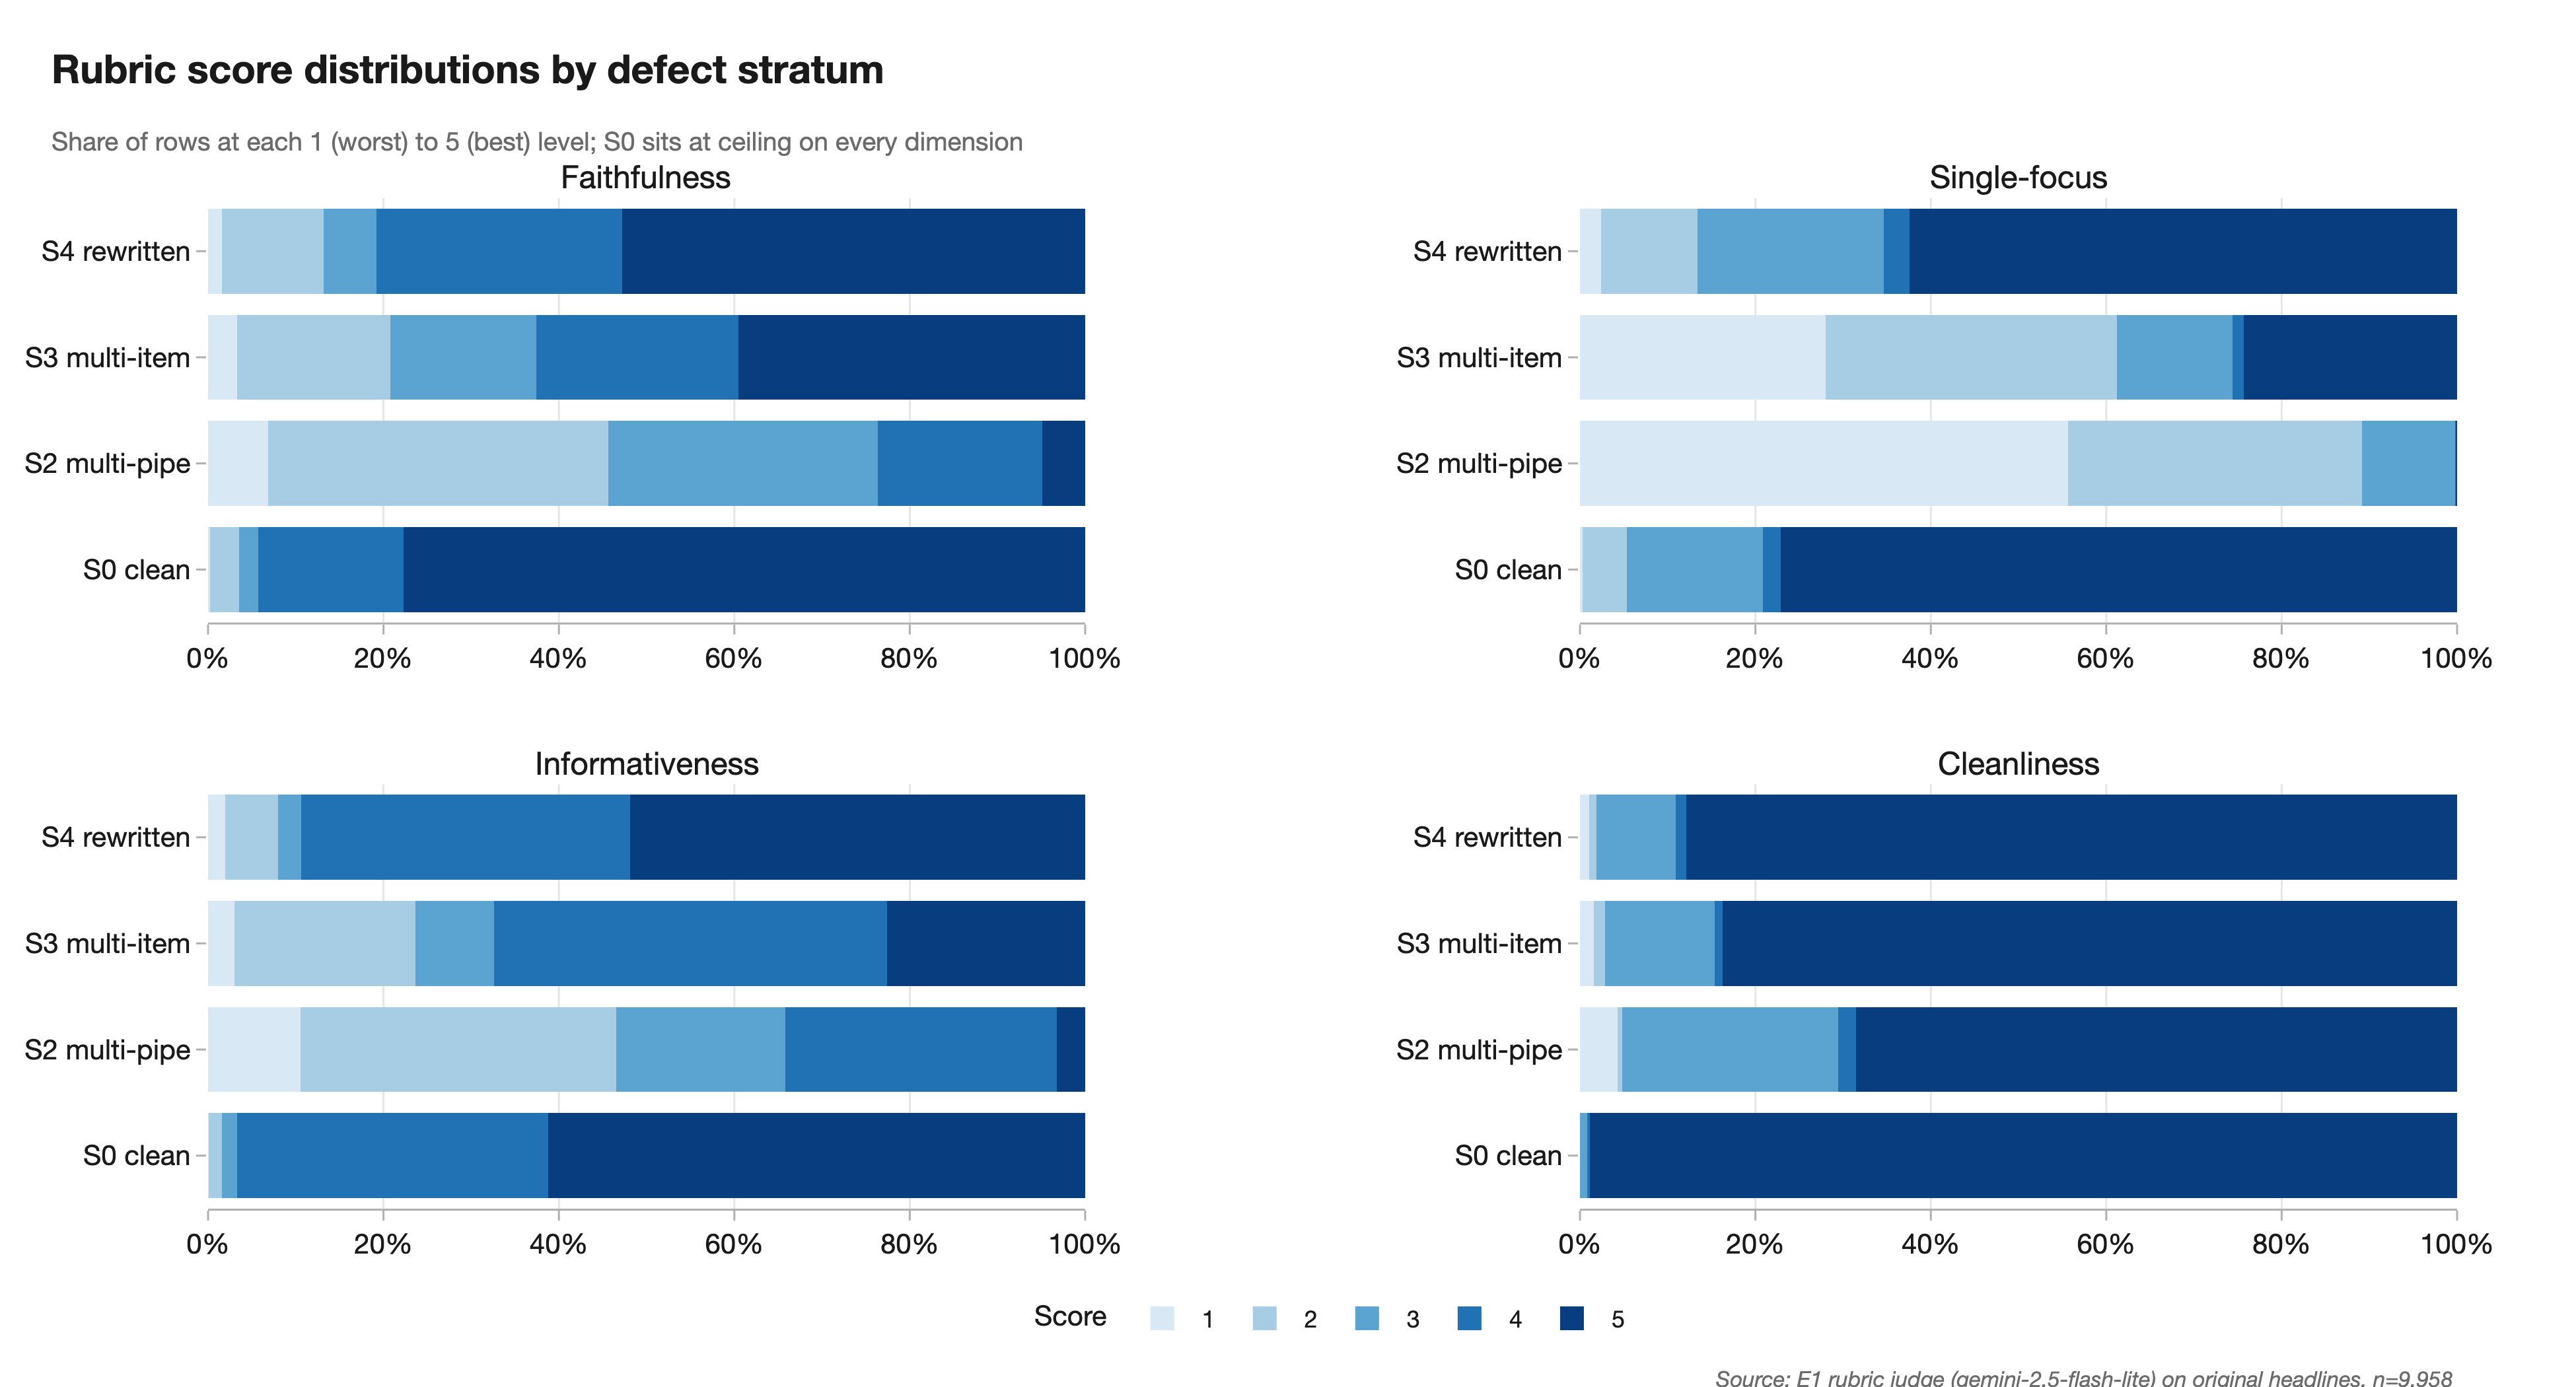
\includegraphics[width=\columnwidth]{figures/f3_rubric_distributions.png}
  \caption{Rubric score distributions by stratum, faceted by dimension. S0 sits at ceiling on every
  dimension; S2 collapses single-focus specifically.}
  \label{fig:e1dist}
\end{figure}

\begin{figure}[t]
  \centering
  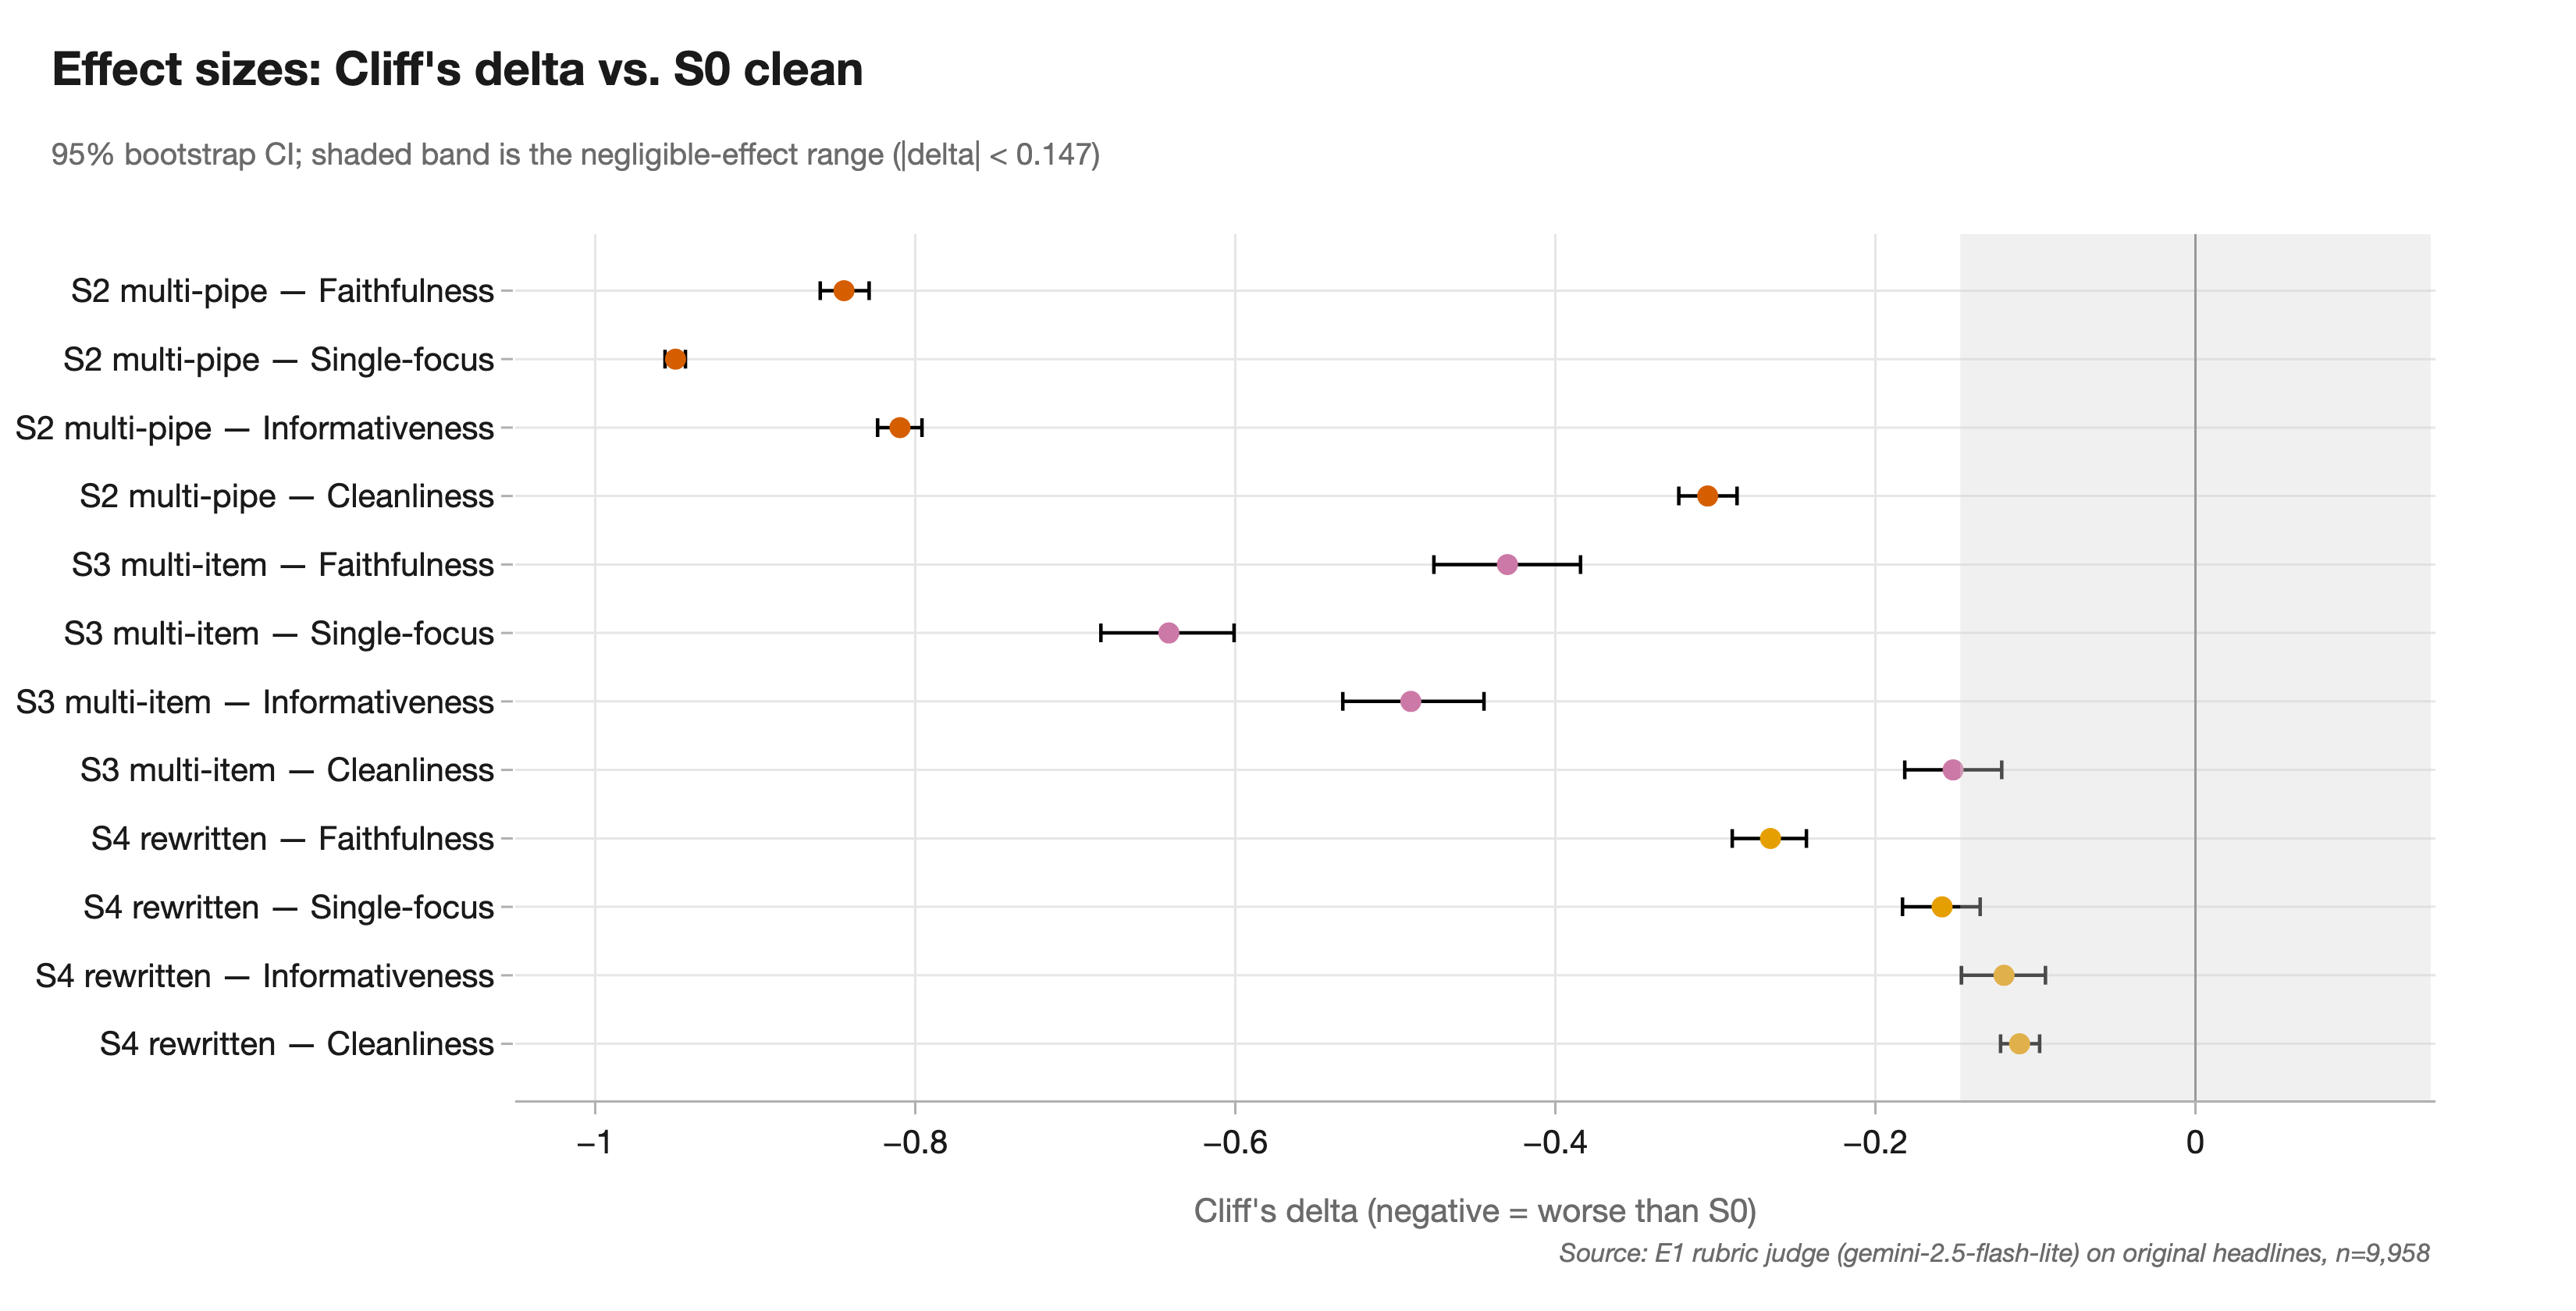
\includegraphics[width=\columnwidth]{figures/f4_effect_sizes.png}
  \caption{Cliff's $\delta$ forest plot with 95\% bootstrap CIs and a shaded negligible band. At
  thousands of rows every comparison is significant, so effect size, not $p$, carries the conclusion.}
  \label{fig:e1delta}
\end{figure}

\subsection{Length and lead bias are continuous, not filter artifacts}
Figure~\ref{fig:f5} regresses the four rubric dimensions and headline--lead word overlap against
$\log(\mathrm{article\ tokens})$ over all $10{,}000$ rows, including the ones the token filter removed.
Headline--lead overlap declines smoothly and monotonically with length, with no discontinuity at the
$4{,}000$-token threshold -- direct support for treating length as a continuous covariate
(Section~\ref{sec:taxonomy}) and the project's lead-bias question in its current form.

\begin{figure}[t]
  \centering
  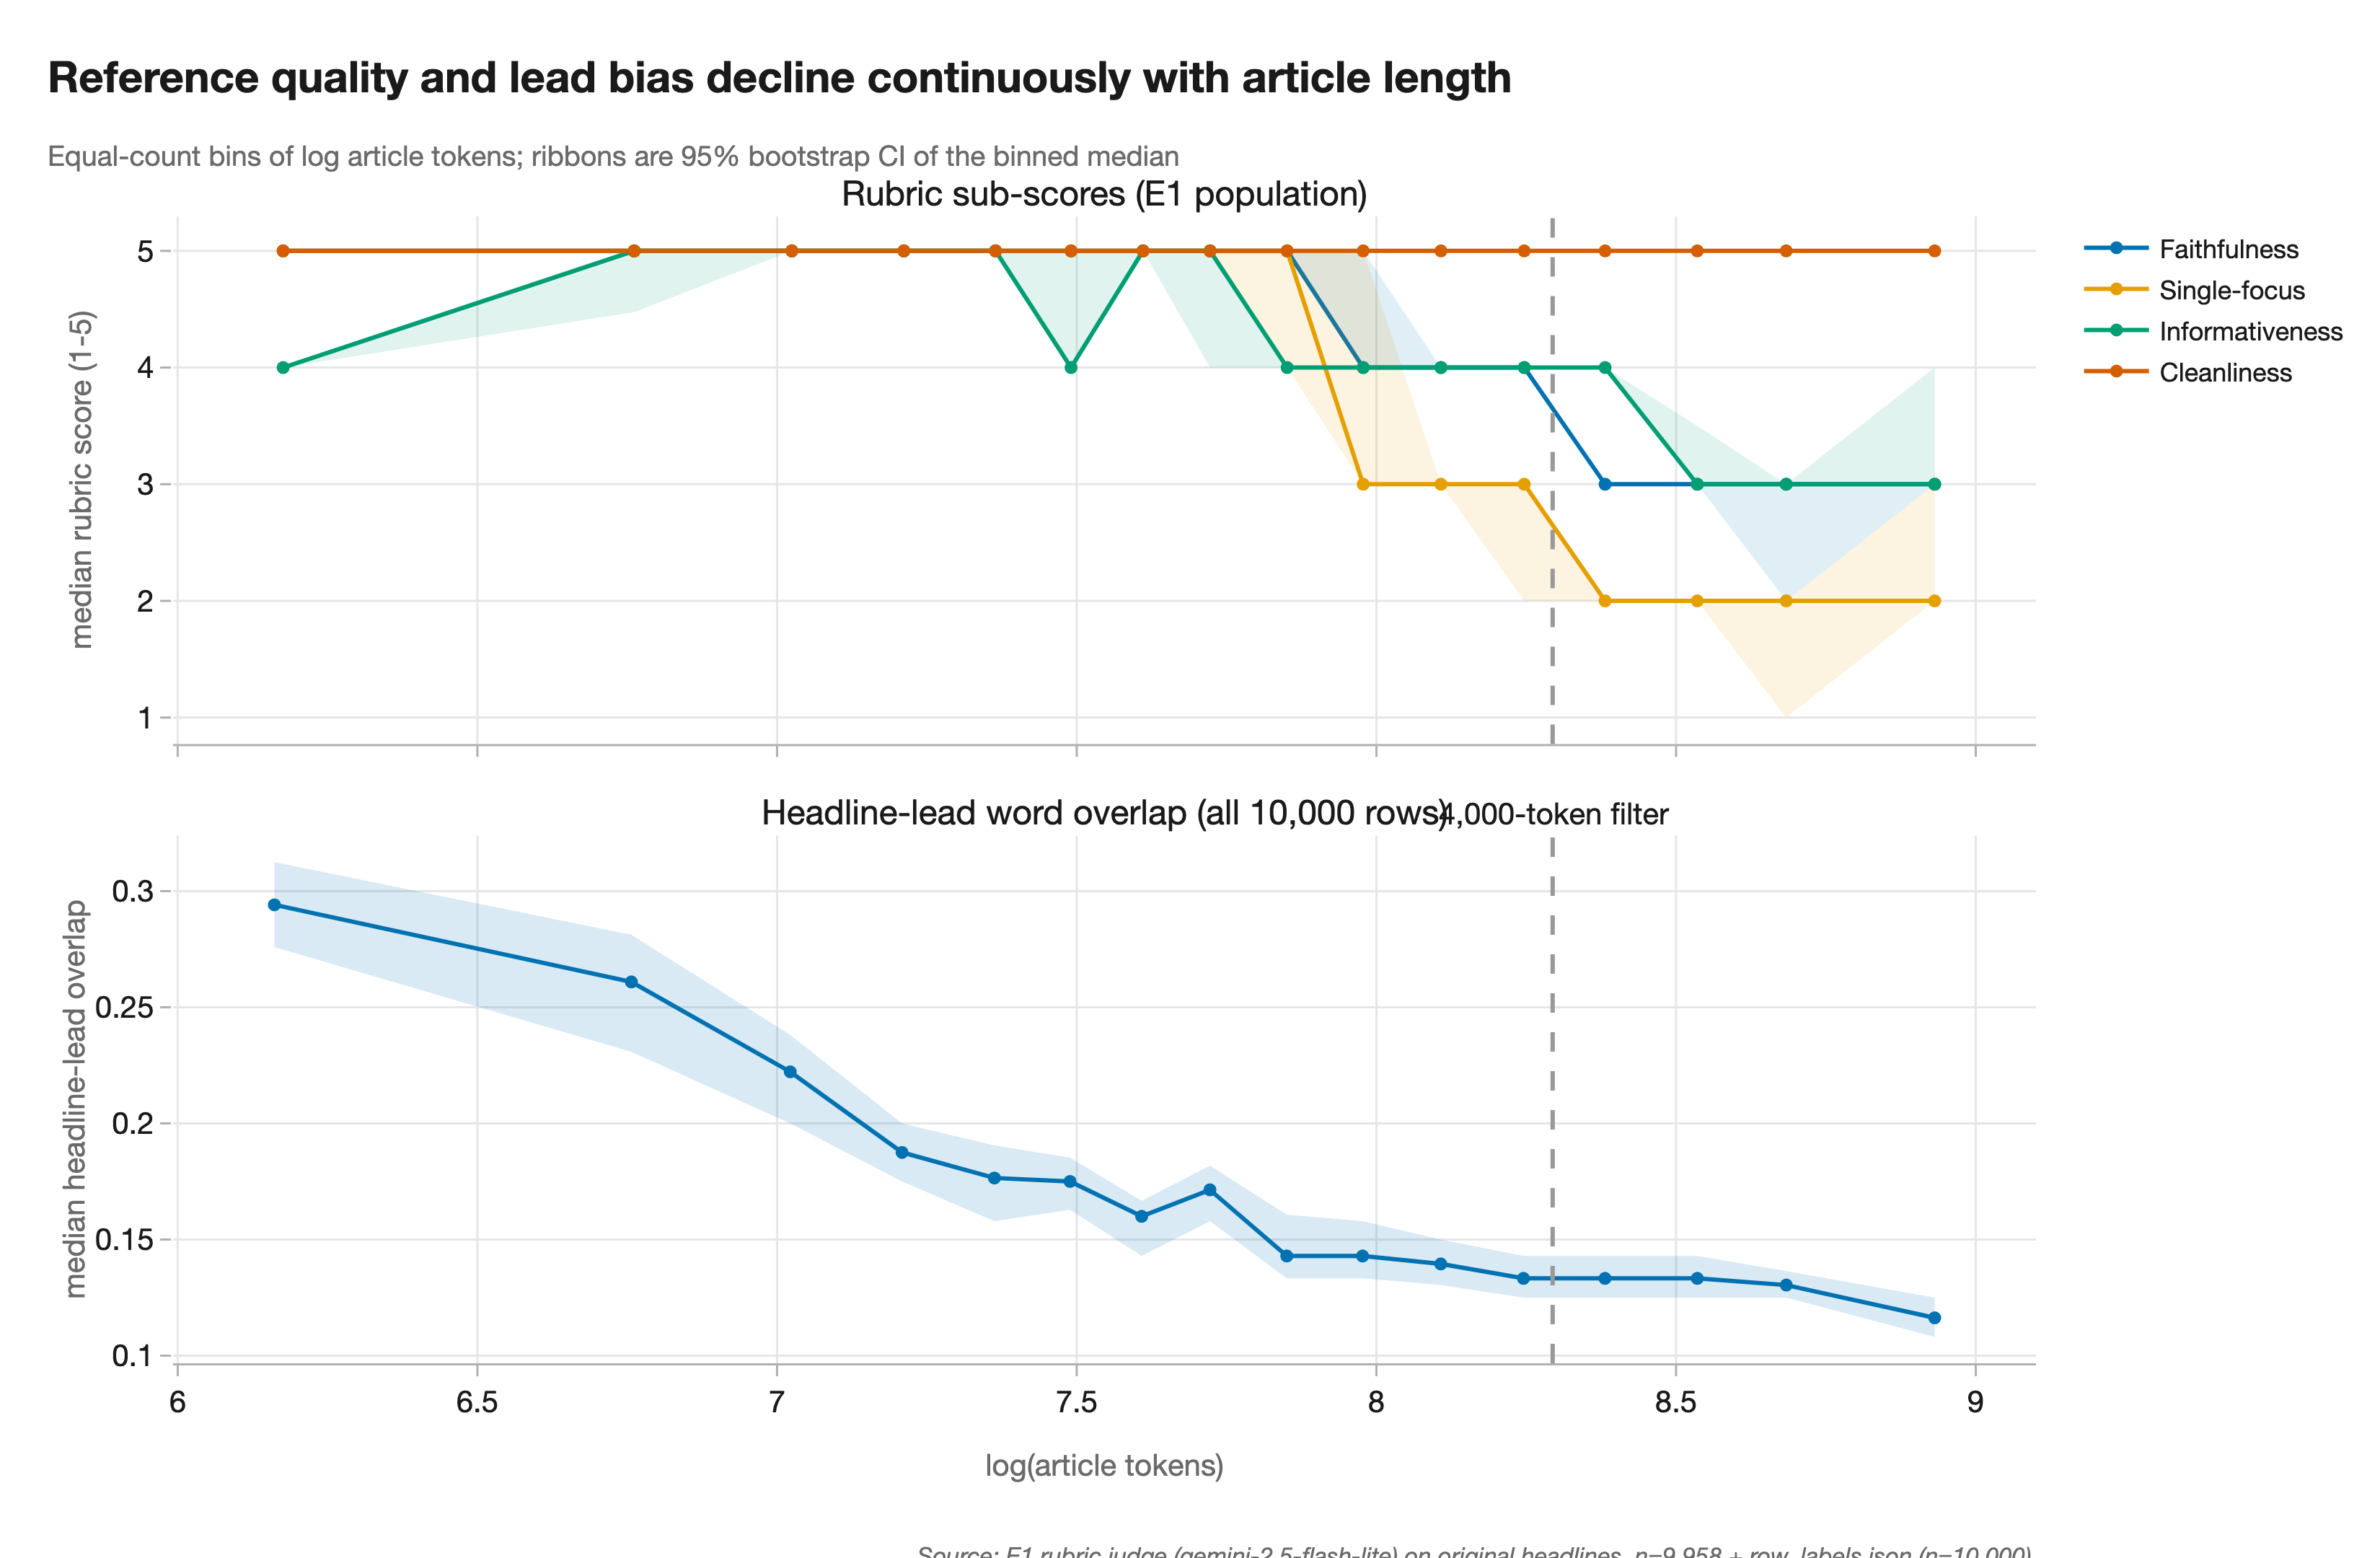
\includegraphics[width=\columnwidth]{figures/f5_length_lead_bias.png}
  \caption{Rubric sub-scores and headline--lead overlap as binned medians over log article length, with
  a vertical rule at the $4{,}000$-token filter threshold.}
  \label{fig:f5}
\end{figure}

\subsection{E2/E3: the repair helped, and the two designs disagree by design}
On the $3{,}068$ paired rewritten rows, every dimension's median sits at ceiling (5.0) both before and
after curation (Figure~\ref{fig:f6}), so the dumbbell plot alone looks flat -- yet the paired Wilcoxon
test is overwhelmingly significant on every dimension (e.g.\ faithfulness: $42.0\%$ of rows increased
vs.\ $3.6\%$ decreased, $p = 8.0\times 10^{-192}$), because many rows move at the top of an ordinal scale
that a median cannot see. This is exactly the ceiling-compression weakness E2 was expected to have, and
it is why we also ran E3.

The blind pairwise comparison (Figure~\ref{fig:f7}) is not compressed: curated headlines are preferred
$73.6\%$ of the time on the rewritten cohort ($n=961$; 95\% CI $[70.8\%, 76.4\%]$), against a
$99.5\%$-tie rate on the untouched placebo cohort ($n=198$). The near-perfect placebo ties validate the
pairwise judge, which makes the $73.6\%$ headline number credible as a real preference rather than
instrument noise. Breaking out by edit sub-type shows the win is concentrated: \texttt{full\_rewrite}
rows ($n{=}833$) are preferred $76.8\%$ of the time, while \texttt{light\_edit} rows ($n{=}97$) are close
to a coin flip ($49.5\%$) -- curation's benefit is real but concentrated in the headlines it changed the
most, not spread evenly across every rewrite. We report E2 and E3 as complementary rather than
contradictory: E2 shows direction and mechanism (which dimension moved), E3 shows magnitude that E2's
scale cannot express.

\begin{figure}[t]
  \centering
  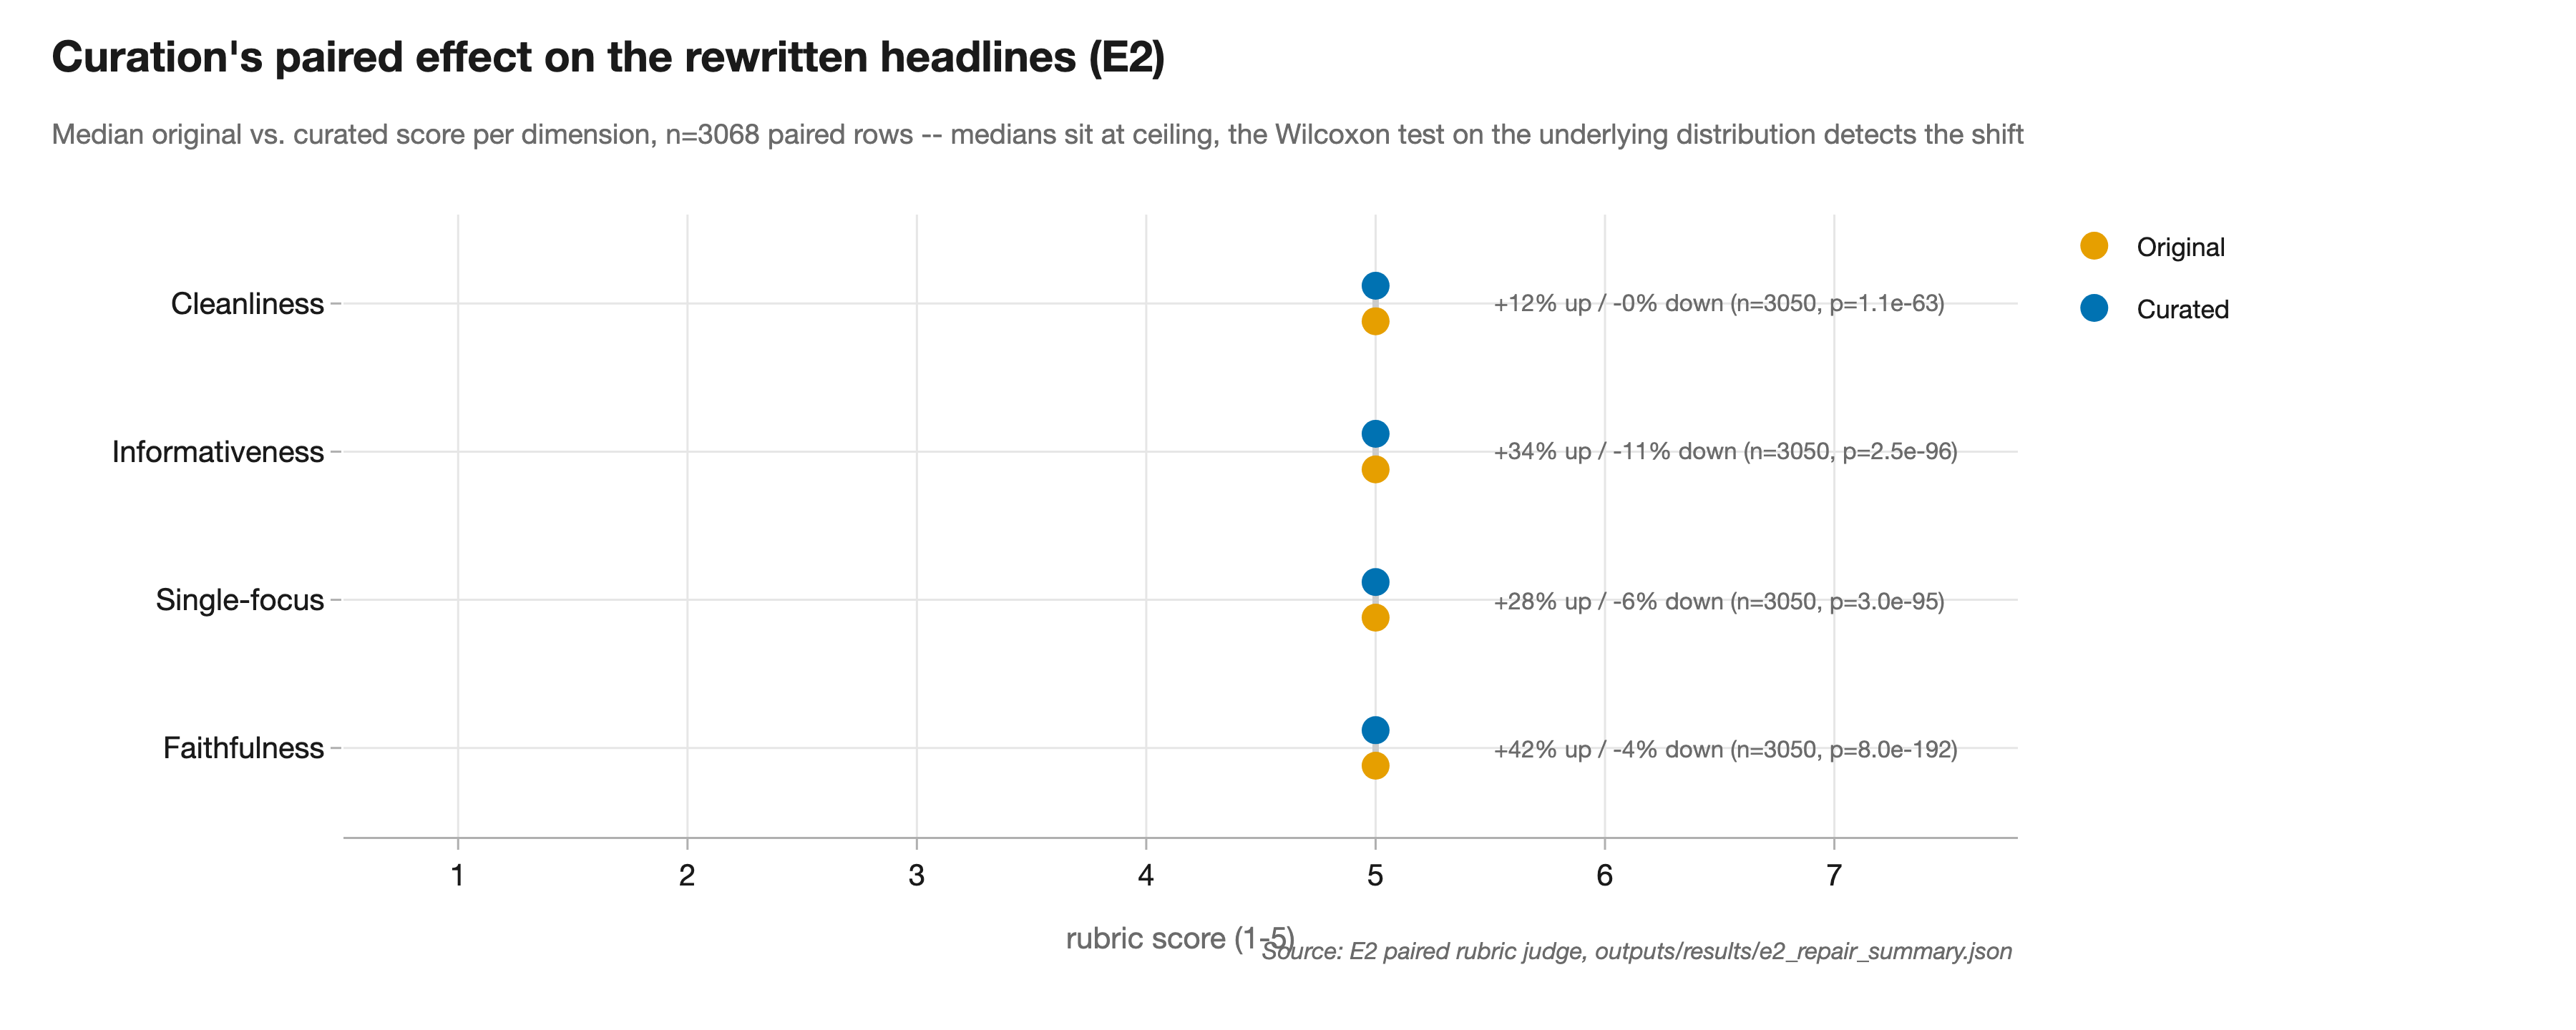
\includegraphics[width=\columnwidth]{figures/f6_paired_repair.png}
  \caption{Paired original-vs-curated median rubric scores over the 3,068 rewritten rows (E2). Medians
  sit at ceiling; the Wilcoxon test on the underlying distributions is what detects the shift.}
  \label{fig:f6}
\end{figure}

\begin{figure}[t]
  \centering
  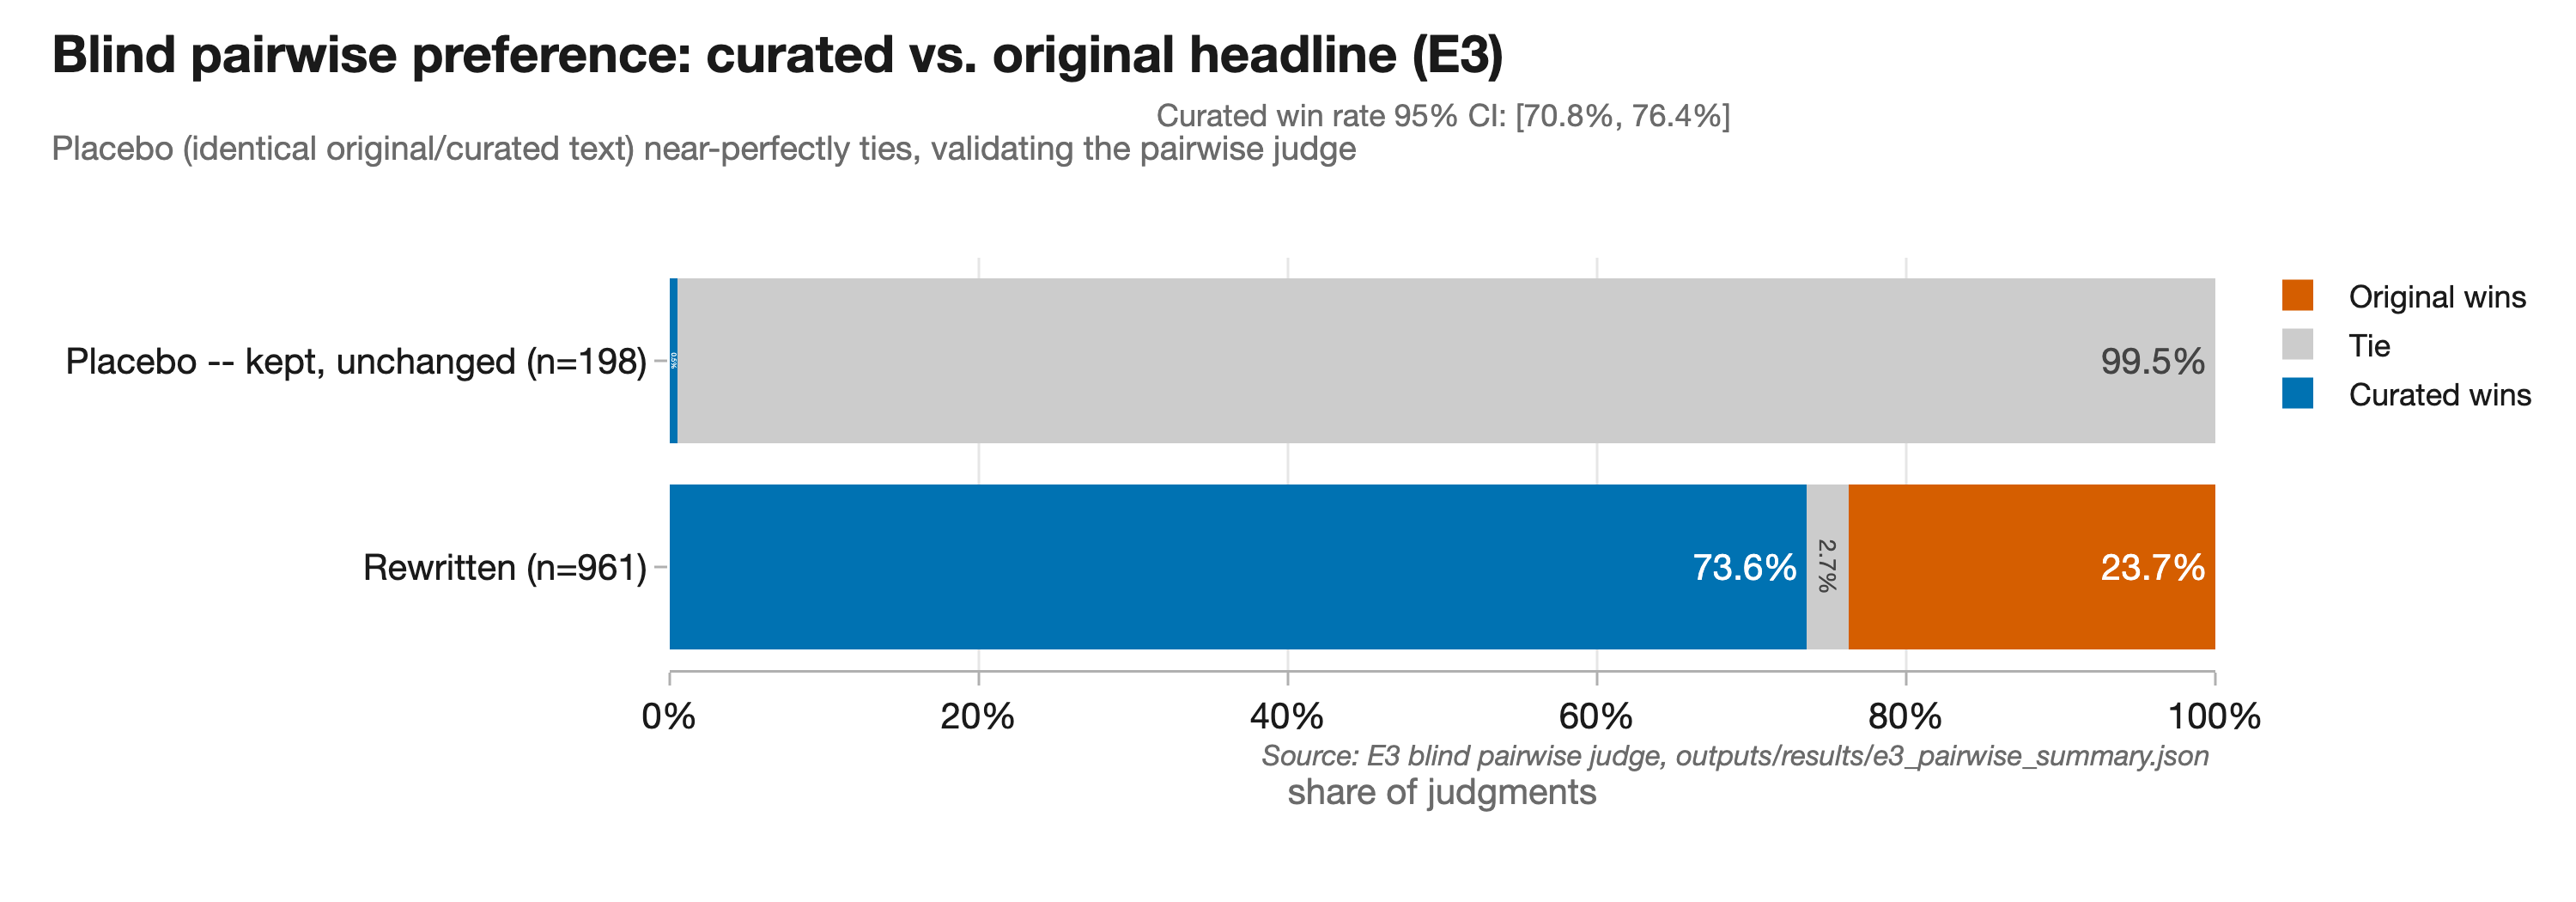
\includegraphics[width=\columnwidth]{figures/f7_win_rate.png}
  \caption{Blind pairwise win rate, curated vs.\ original, with the placebo drawn in the same figure
  (E3).}
  \label{fig:f7}
\end{figure}

\subsection{Zero-shot model output vs.\ reference on the same rubric axis}
As a model-driven check that does not depend on the fine-tuning run in progress, Figure~\ref{fig:f9}
compares zero-shot \texttt{dictalm2.0-instruct} outputs against the reference headline on the identical
rubric axis, over $604$ of a planned $800$-row stratified sample (inference incomplete at submission
time). The clearest result is a \textbf{reversal}: on S2 multi-pipe rows, the zero-shot model is
\emph{more single-focus} than the reference it is being compared against (median 2 vs.\ 1,
$\delta = +0.41$) -- direct evidence that a defective reference can score worse than a generic
summarizer on exactly the dimension the defect damages. S0's large faithfulness gap (reference median 5
vs.\ model median 2) is not a comparable finding: it is largely a headline-length-vs-summary-length
format mismatch, since the model was not instructed to write in a headline register, and we report it
as a confound rather than a "model beats gold" claim.

\begin{figure}[t]
  \centering
  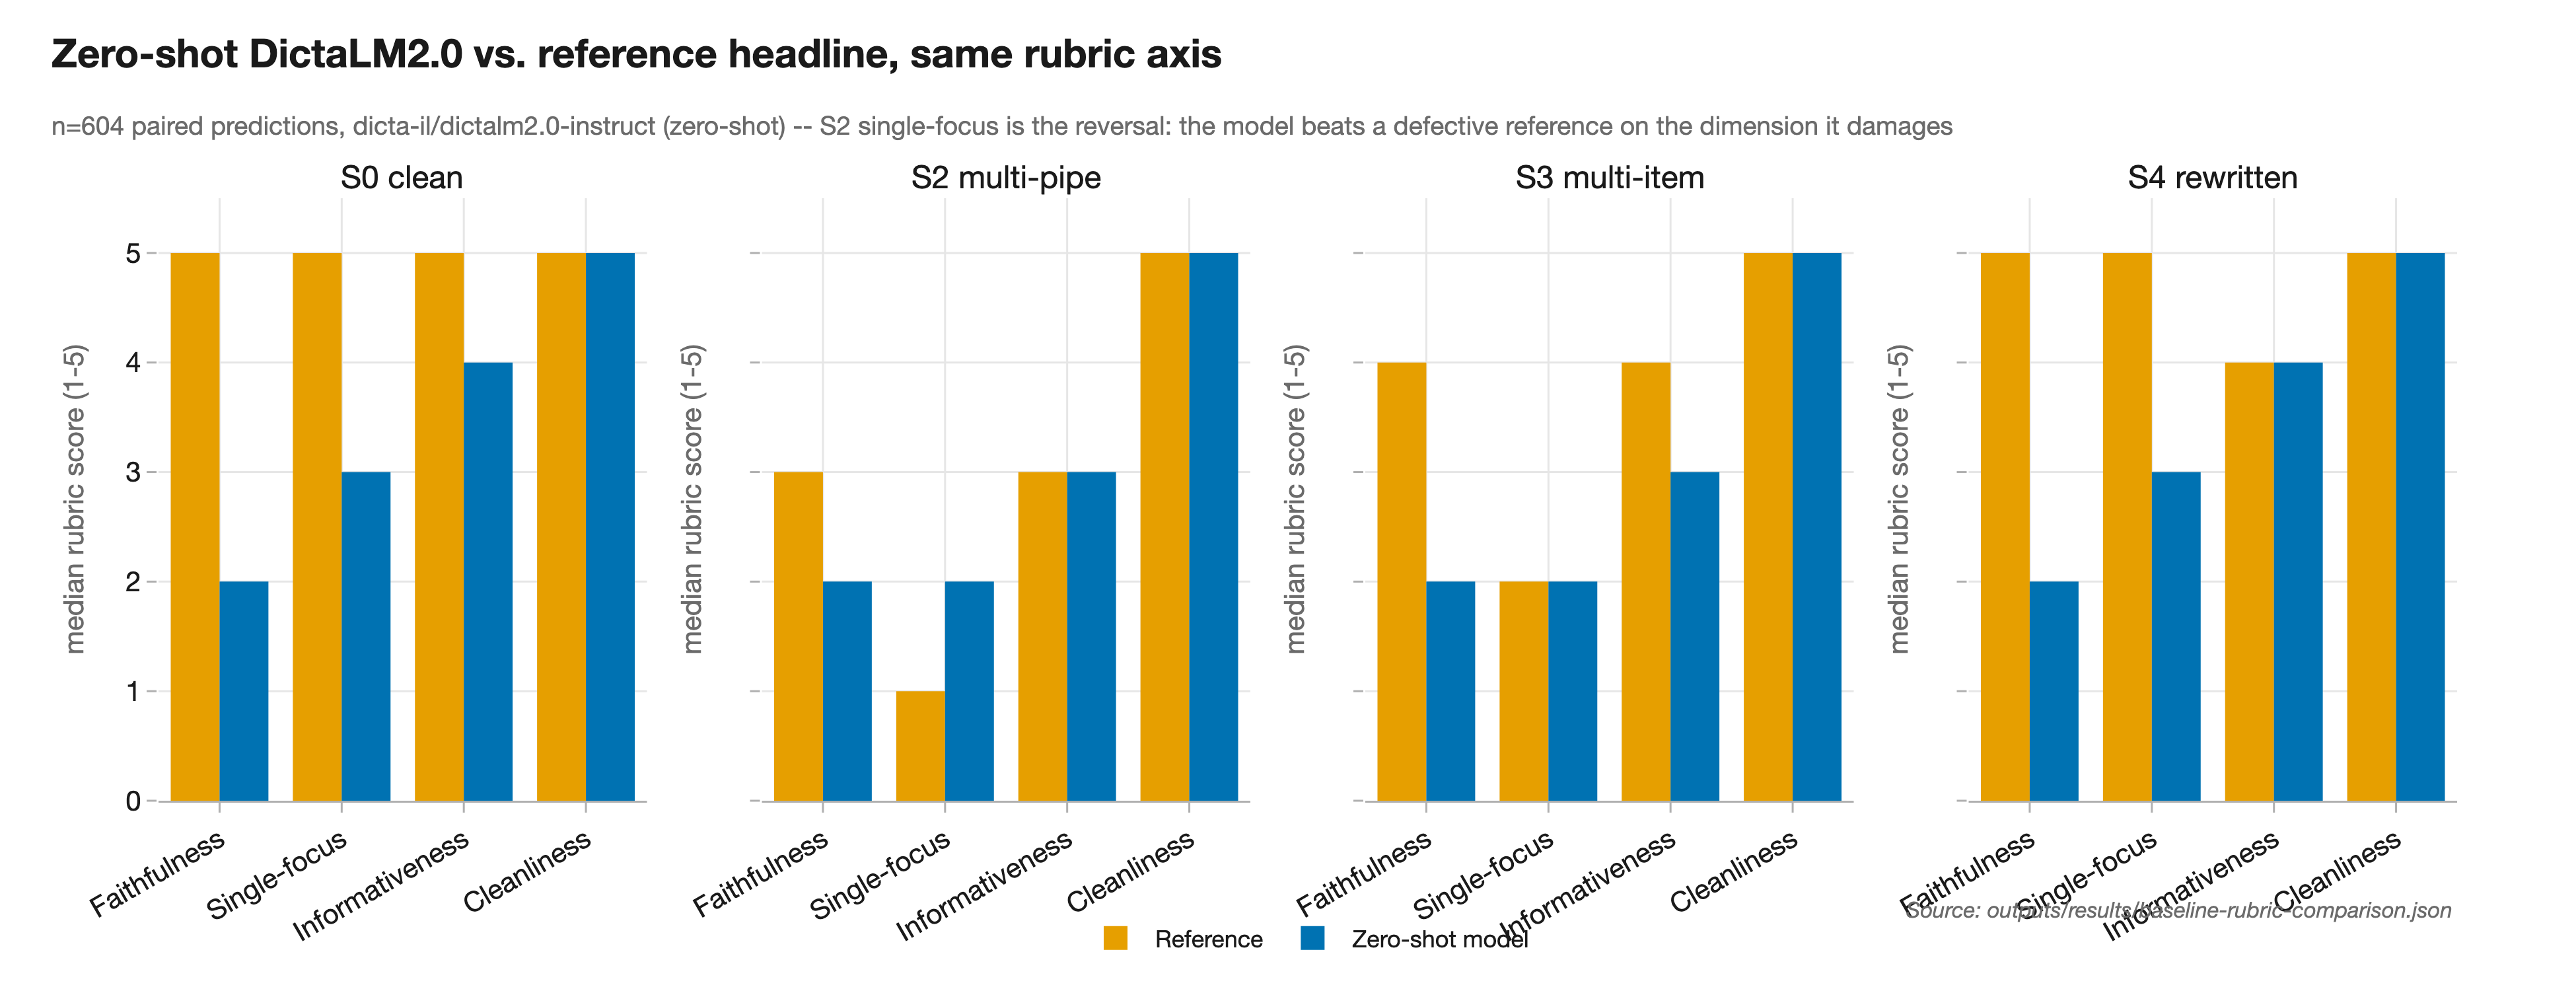
\includegraphics[width=\columnwidth]{figures/f9_baseline_vs_reference_rubric.png}
  \caption{Zero-shot DictaLM2.0 output vs.\ reference headline, median rubric score by stratum
  ($n=604$, partial).}
  \label{fig:f9}
\end{figure}

\subsection{E4: training comparison (in progress)}
\label{sec:e4-results}
At submission time the Arm B fine-tuning job had completed $275$ of $293$ steps ($\sim\!94\%$ of one
epoch) before an infrastructure error, with its adapter already pushed and inference now at $580$ of
$586$ test-set predictions (Appendix~\ref{app:finetuned-interim} reports an early, explicitly-labeled
look at this partial checkpoint). Arm A training had not yet started. We therefore report the
comparison's \emph{skeleton} rather than results: once both arms' predictions land on the frozen test
split, Figure~\ref{fig:f8-placeholder} will be replaced by (i) grouped rubric-score bars for Arm A and
Arm B on the same four dimensions as Figure~\ref{fig:e1dist}, and (ii) a blind pairwise Arm A vs.\ Arm B
win rate under the same placebo design as Figure~\ref{fig:f7}. We record in advance which conclusions
survive if fewer arms complete than planned: with both arms, the full causal claim about curation is
available; with Arm B alone, nothing about curation follows and the paper's contribution falls back
entirely on the audit in E1--E3, which never depended on training and stands on its own.

\begin{figure}[t]
  \centering
  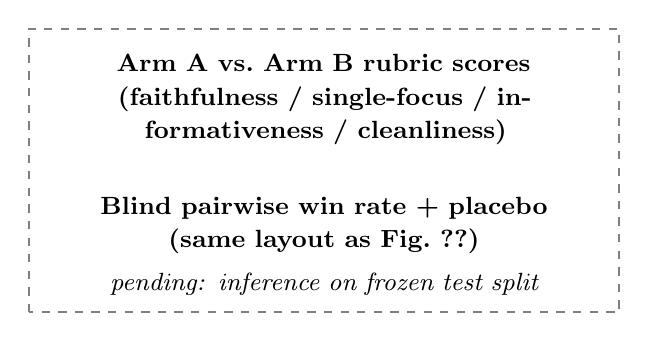
\begin{tikzpicture}
    \draw[dashed, thick, gray] (0,0) rectangle (7.5,3.6);
    \node[align=center, text width=6.8cm] at (3.75,2.7)
      {\small\bfseries Arm A vs.\ Arm B rubric scores\\ \small(faithfulness / single-focus /
      informativeness / cleanliness)};
    \node[align=center, text width=6.8cm] at (3.75,1.1)
      {\small\bfseries Blind pairwise win rate + placebo\\ \small(same layout as Fig.~\ref{fig:f7})};
    \node[align=center, text width=6.8cm, font=\small\itshape] at (3.75,0.35)
      {pending: inference on frozen test split};
  \end{tikzpicture}
  \caption{Planned layout for the E4 before/after comparison. Populated once Arm A and Arm B
  predictions are both available on the frozen test split (Section~\ref{sec:e4-results}).}
  \label{fig:f8-placeholder}
\end{figure}

\subsection{Limitations}
The rubric judge and the curator are different model families by design, but neither is a human gold
standard; a 150-row human validation round is planned but not yet run
(Appendix~\ref{app:pilot} reports the cheaper test--retest check in the meantime). The external
fine-tuning job's Hub-hosted test split ($586$ rows, no persisted row id) does not yet provably align
with our reconstructed frozen split ($1{,}162$ ids); resolving this id recovery is a precondition for
E4, not merely a formatting detail. The zero-shot baseline in Figure~\ref{fig:f9} is scored on a partial
sample and its S0 faithfulness gap reflects a headline-vs-summary length confound rather than a clean
comparison. Finally, this design tests whether \emph{repairing} a flagged headline helps; it does not by
itself establish whether \emph{dropping} the $\sim\!4{,}146$ filtered-out rows was the right call, since
neither training arm trains on them -- that remains open for a future arm that reintroduces filtered
rows under curated headlines.

\clearpage

% Additional tables and figures beyond the main body

\begin{table}[t]
\centering
\small
\begin{tabular}{lrrl}
\hline
\textbf{Stage} & \textbf{Input} & \textbf{Output} & \textbf{Effect} \\
\hline
Download & -- & 10{,}000 & baseline \\
Tail trim & 10{,}000 & 10{,}000 & 722 tails removed \\
Token budget & 10{,}000 & 7{,}341 & 2{,}659 removed \\
Multi-pipe & 10{,}000 & 7{,}588 & 2{,}412 removed \\
Intersection & -- & 6{,}486 & 35.1\% removed \\
Source filter & 6{,}486 & 5{,}854 & 632 unusable \\
Headline curation & 5{,}854 & 5{,}854 & 3{,}069 rewritten \\
\hline
\end{tabular}
\caption{Curation pipeline counts, verified against artifacts on disk (Section~\ref{sec:data}).}
\label{tab:pipeline}
\end{table}

\appendix

\section{Qwen3-2B fine-tuning history}
\label{app:qwen}
Retained for the record; superseded by the dataset review in the main paper. Three training iterations,
each fixing the previous one's diagnosis (Section~\ref{sec:pivot}):

\begin{table}[h]
\centering
\small
\begin{tabular}{lrrrr}
\toprule
\textbf{Version} & \textbf{R-1} & \textbf{R-2} & \textbf{R-L} & \textbf{BERTScore F1} \\
\midrule
v1 (1ep, attn-only LoRA) & 11.4 & 4.5 & 9.2 & 0.449 \\
v2 (v1 adapter, new decode) & 4.7 & 0.2 & 3.7 & 0.383 \\
v3 (3ep, full LoRA) & 5.1 & 0.3 & 4.0 & 0.390 \\
\bottomrule
\end{tabular}
\caption{Qwen3-2B ROUGE and AlephBERT BERTScore F1 across three fixes. The v1$\to$v2 drop is a
repetition artifact being suppressed, not a real regression; v3's judge-rated faithfulness (2.64)
remained below the untuned base model's (2.98), the finding that ended this era.}
\label{tab:qwen}
\end{table}

\section{Rubric instrument validation}
\label{app:pilot}
Figure~\ref{fig:kappa} shows test--retest quadratically weighted Cohen's $\kappa$ per dimension from the
300-row pilot (Section~\ref{sec:methods}); Figure~\ref{fig:filteroverlap} shows the overlap between the
two deterministic filters referenced in Section~\ref{sec:data}.

\begin{figure}[h]
  \centering
  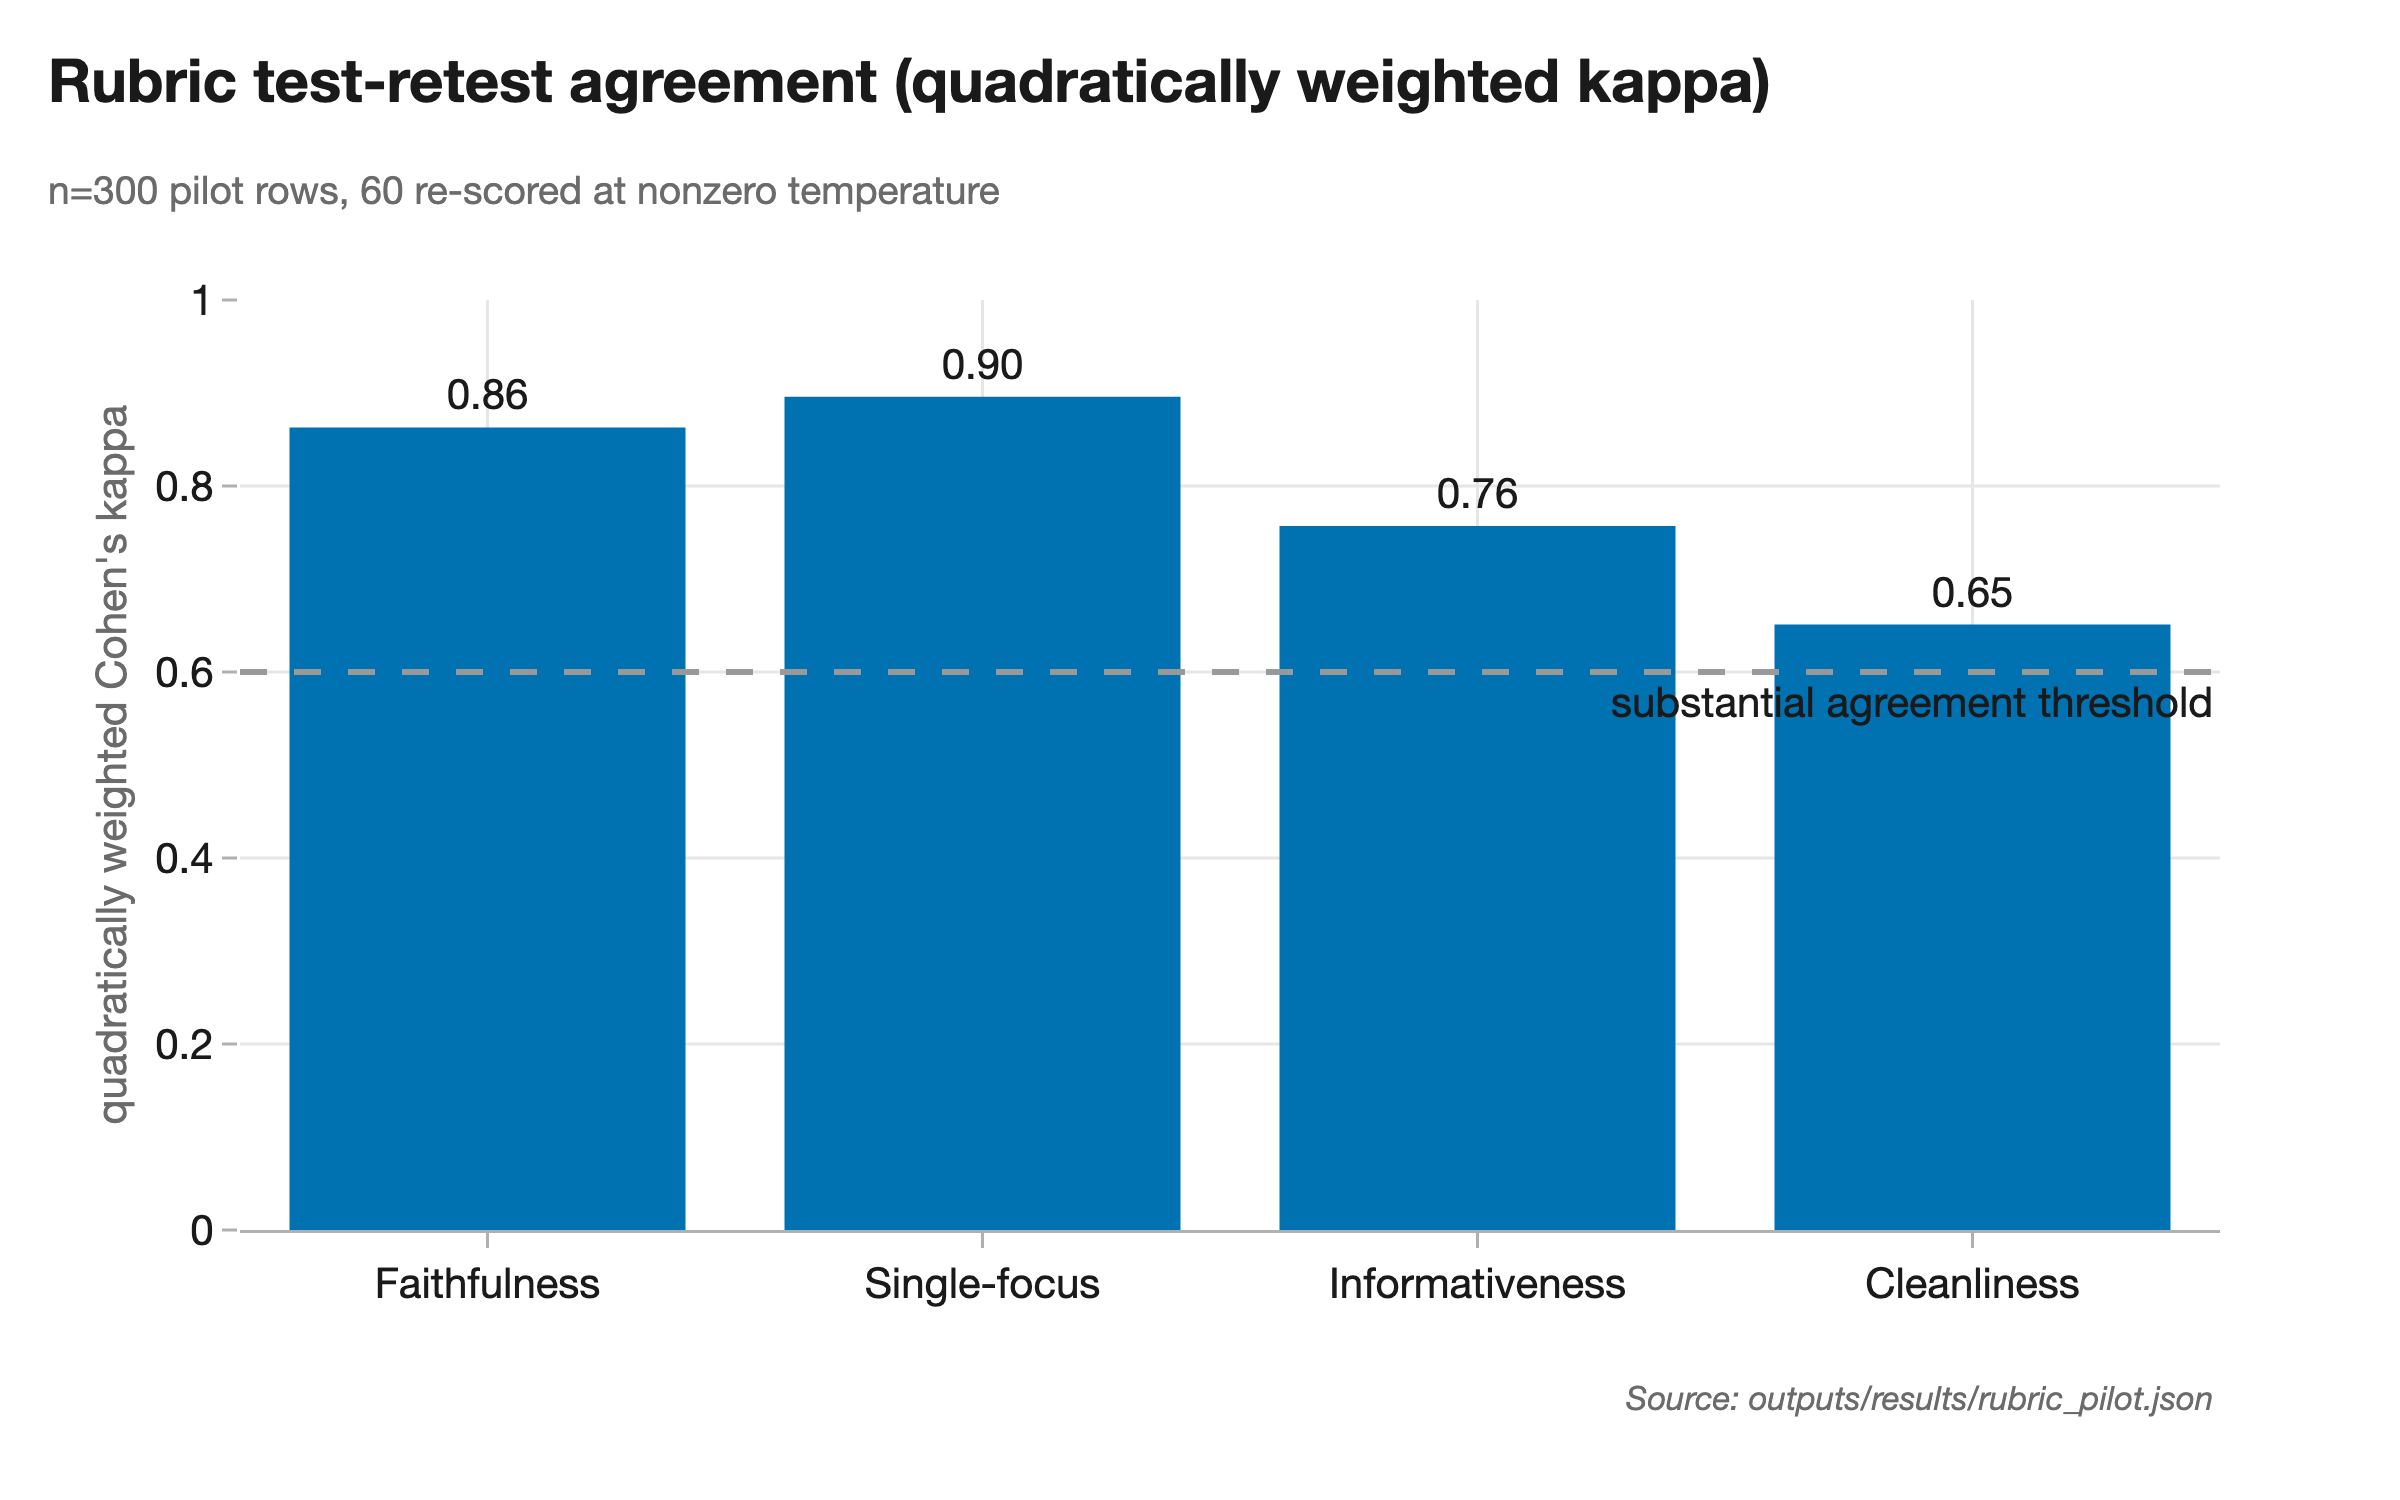
\includegraphics[width=\columnwidth]{figures/sx16_pilot_kappa.png}
  \caption{Test--retest agreement (quadratically weighted $\kappa$) per rubric dimension.}
  \label{fig:kappa}
\end{figure}

\begin{figure}[h]
  \centering
  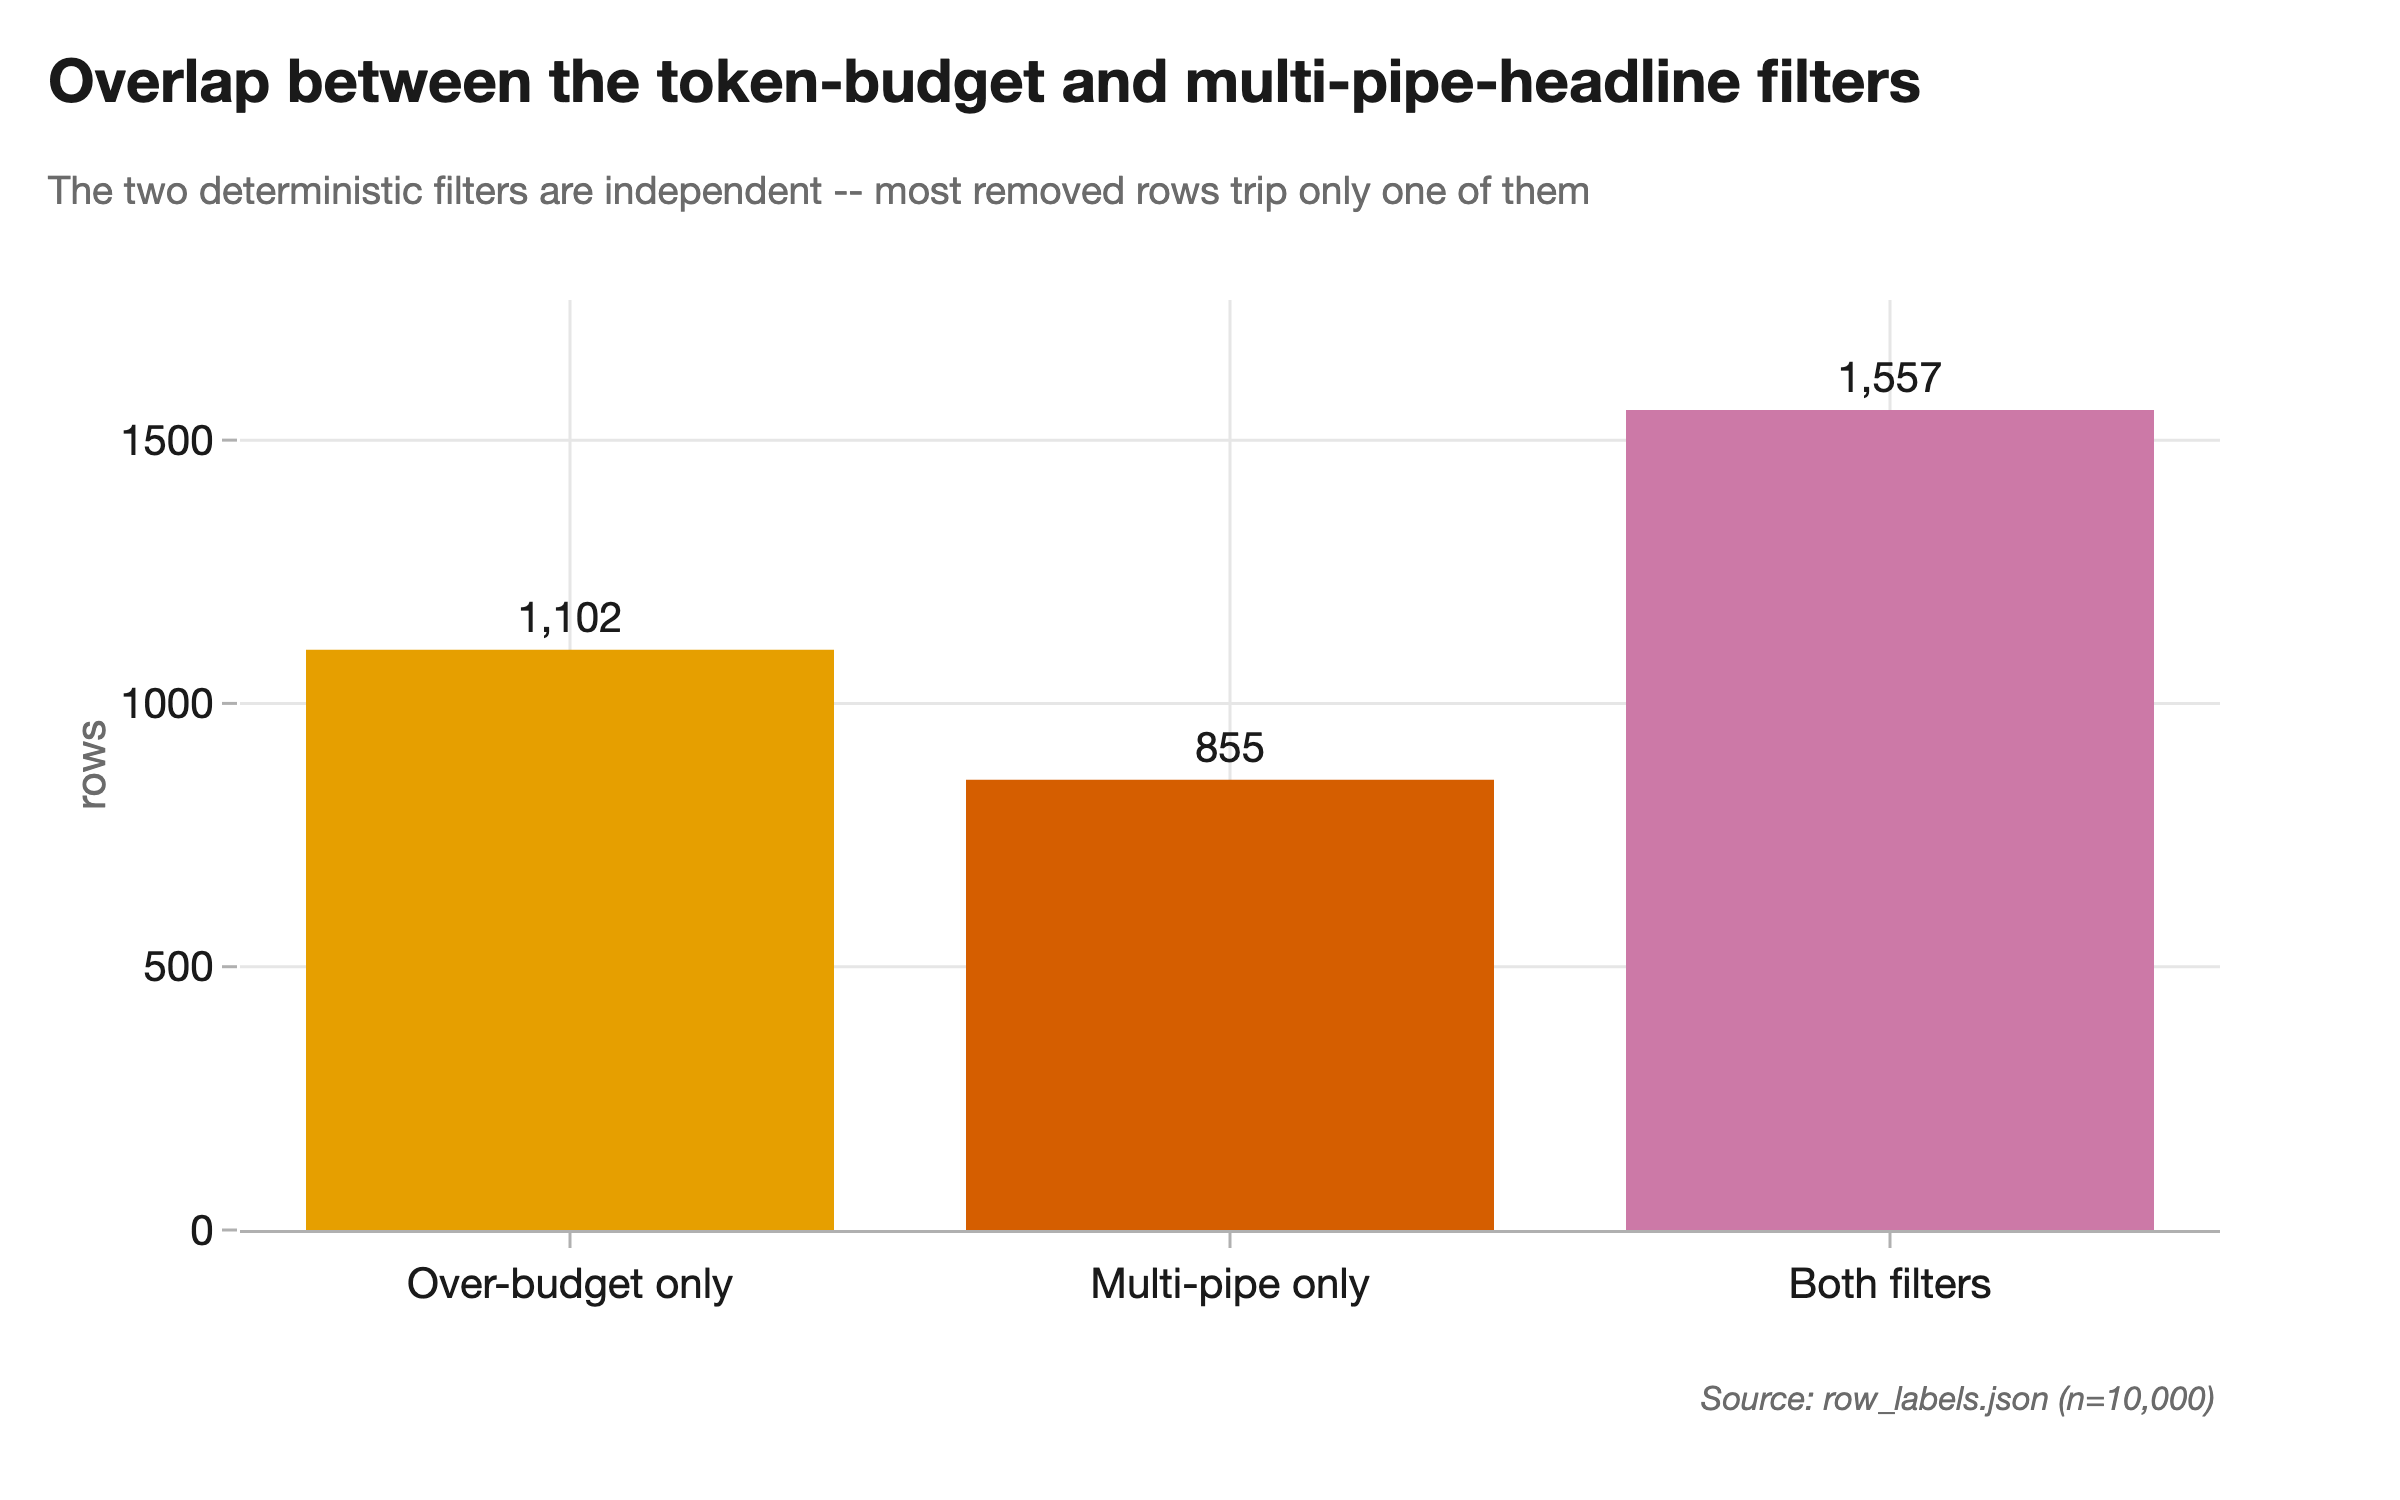
\includegraphics[width=\columnwidth]{figures/sx01_filter_overlap.png}
  \caption{Overlap between the token-budget and multi-pipe-headline filters.}
  \label{fig:filteroverlap}
\end{figure}

\section{Headline edit sub-types}
\label{app:subtypes}
The $3{,}069$ rewrites are sub-typed post hoc from the (original, replacement) string pair alone
(Figure~\ref{fig:subtypes}): \texttt{pipes\_removed}, \texttt{boilerplate\_stripped},
\texttt{truncation\_repaired}, \texttt{light\_edit}, and \texttt{full\_rewrite}, first match wins. The
E3 win-rate split by sub-type (Section~\ref{sec:results}) shows the repair's benefit concentrates in
\texttt{full\_rewrite}.

\begin{figure}[h]
  \centering
  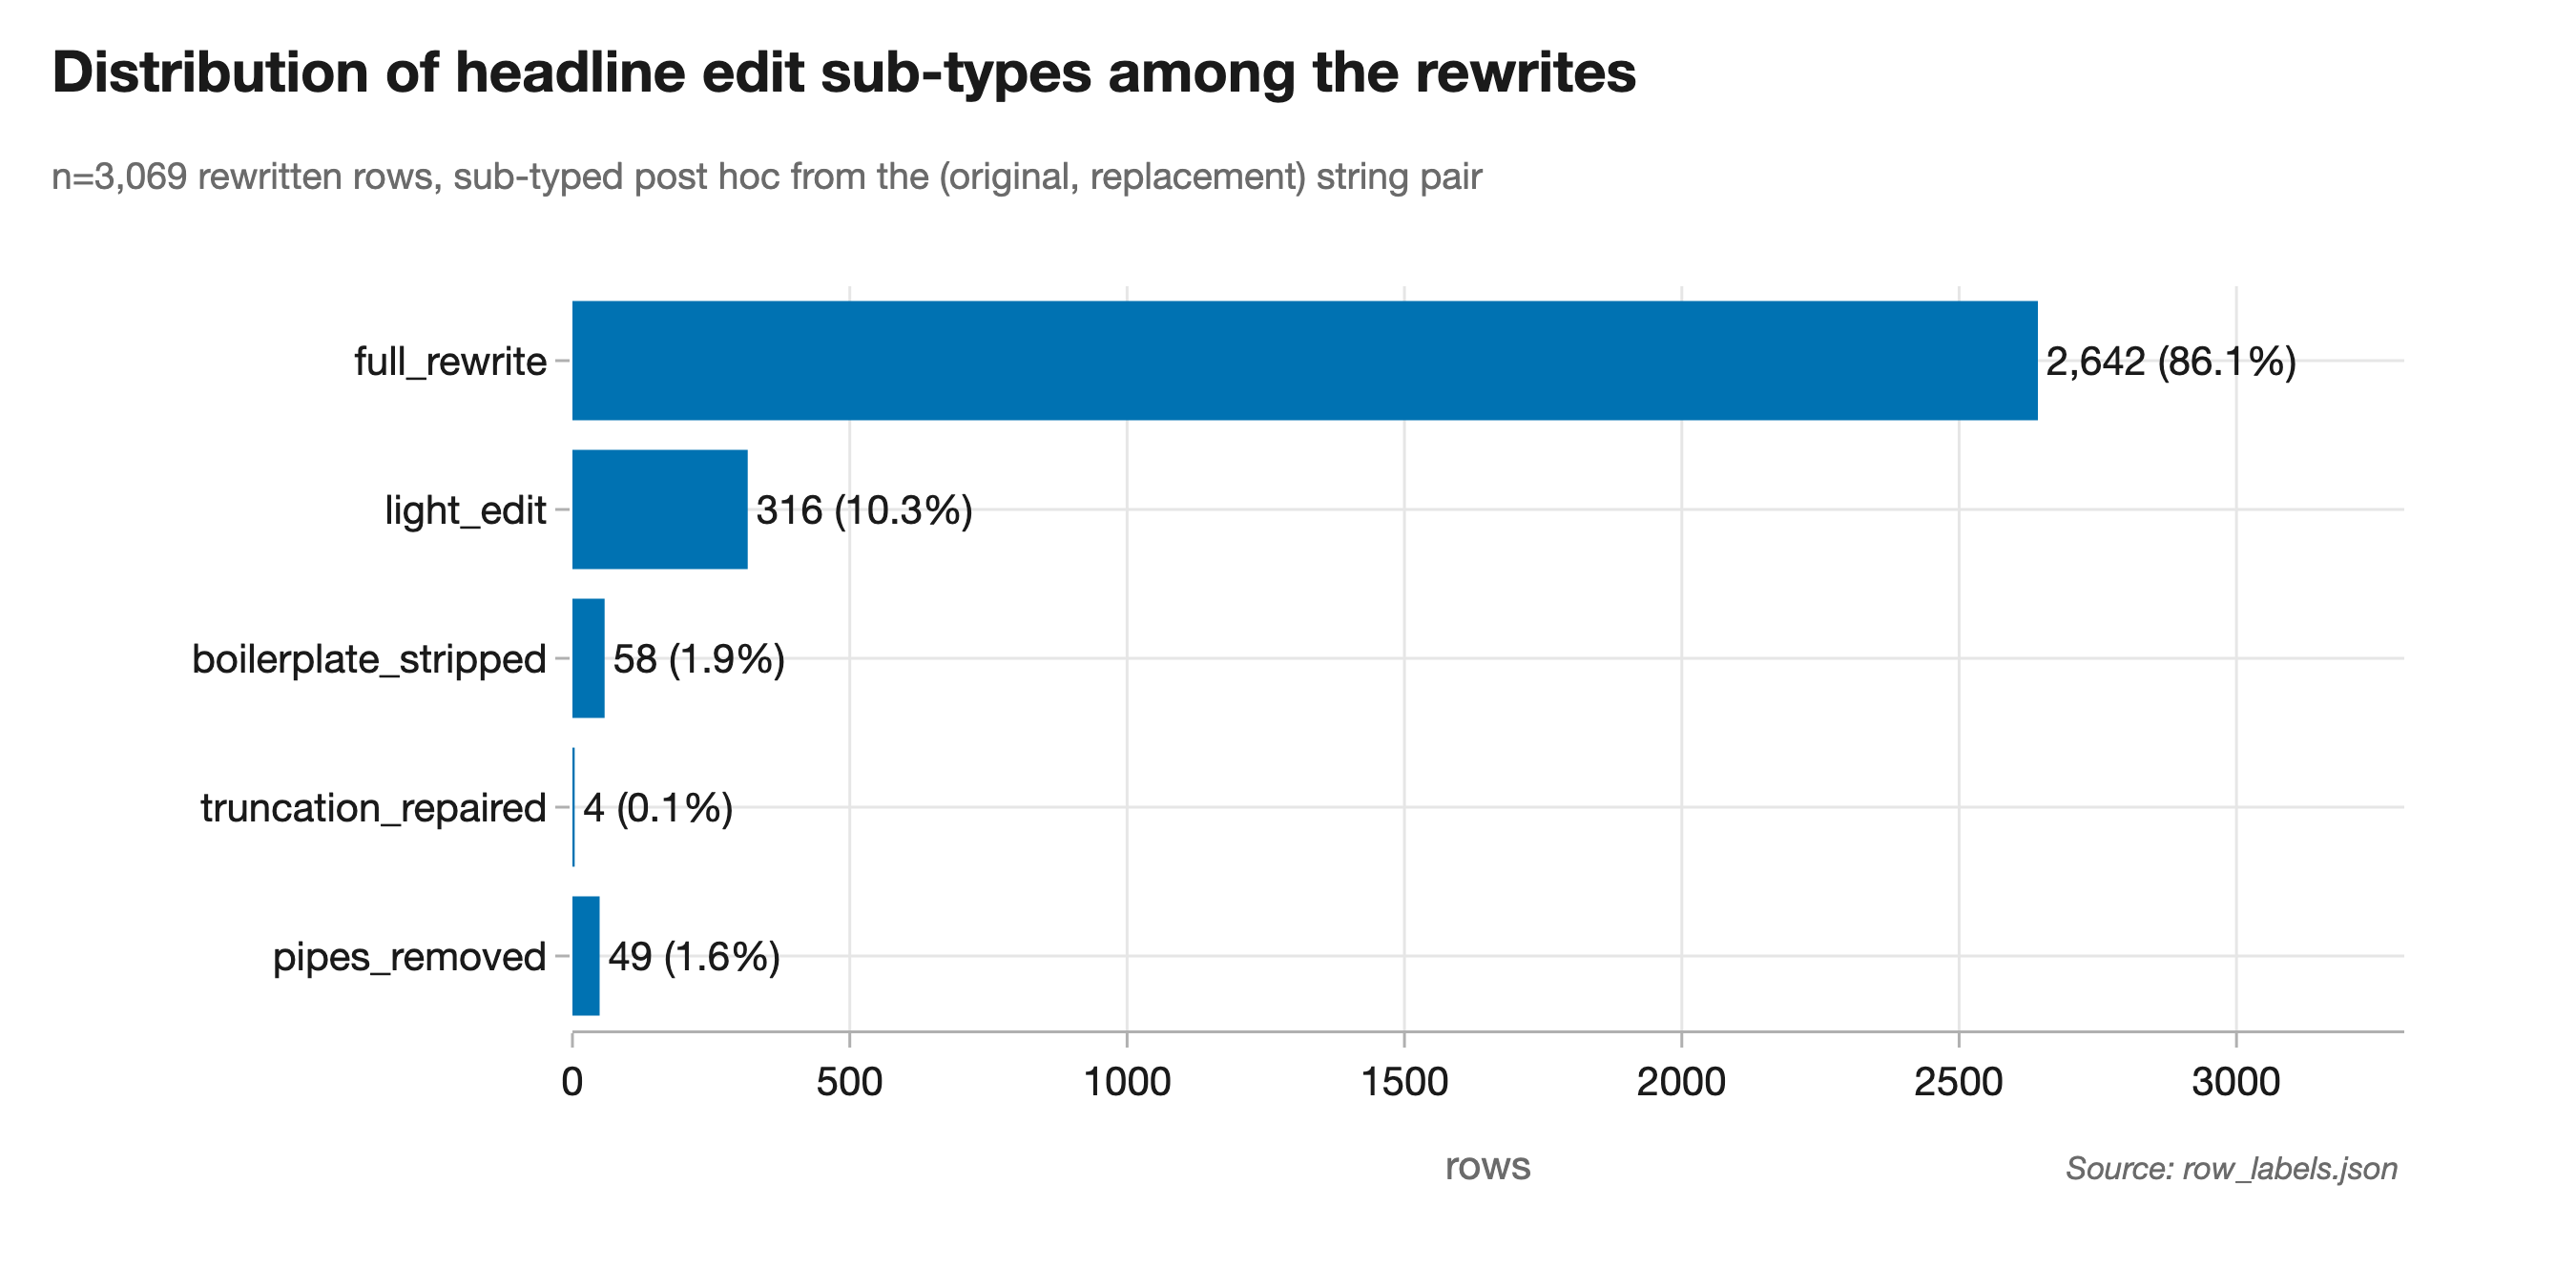
\includegraphics[width=\columnwidth]{figures/sx05_headline_edit_subtypes.png}
  \caption{Distribution of headline edit sub-types among the 3,069 rewrites.}
  \label{fig:subtypes}
\end{figure}

\section{Dual-reference zero-shot probe}
\label{app:probe}
As a metric-based triangulation independent of the rubric judge, \texttt{DictaLM-3.0-1.7B-Instruct}
generates one zero-shot prediction per article ($n=1{,}427$, stratified subsample) and that same
prediction is scored twice: once against the original headline, once against the curated one. Because
the prediction never changes, any ROUGE/BERTScore gap is attributable only to which reference was used.
The placebo group (\texttt{kept}, where curation left the headline untouched) shows an exact
$0.0$ median gap ($p=1.0$), confirming the method is not picking up scoring noise; the \texttt{all}-row
gap is small (mean ROUGE-1 gap $-0.0026$) and in the direction that favors the original wording over
the curated one, which is the expected behavior of a lexical-overlap metric that rewards surface
similarity rather than quality -- the reason ROUGE is not used as a primary instrument in this paper.

\section{Repair transition detail}
\label{app:transition}
Figure~\ref{fig:transition} is the transition heatmap referenced in Section~\ref{sec:results}: original
score against curated score for the dimension that moved most (faithfulness), showing where mass moved
and confirming it moved almost entirely toward higher scores rather than lower ones.

\begin{figure}[h]
  \centering
  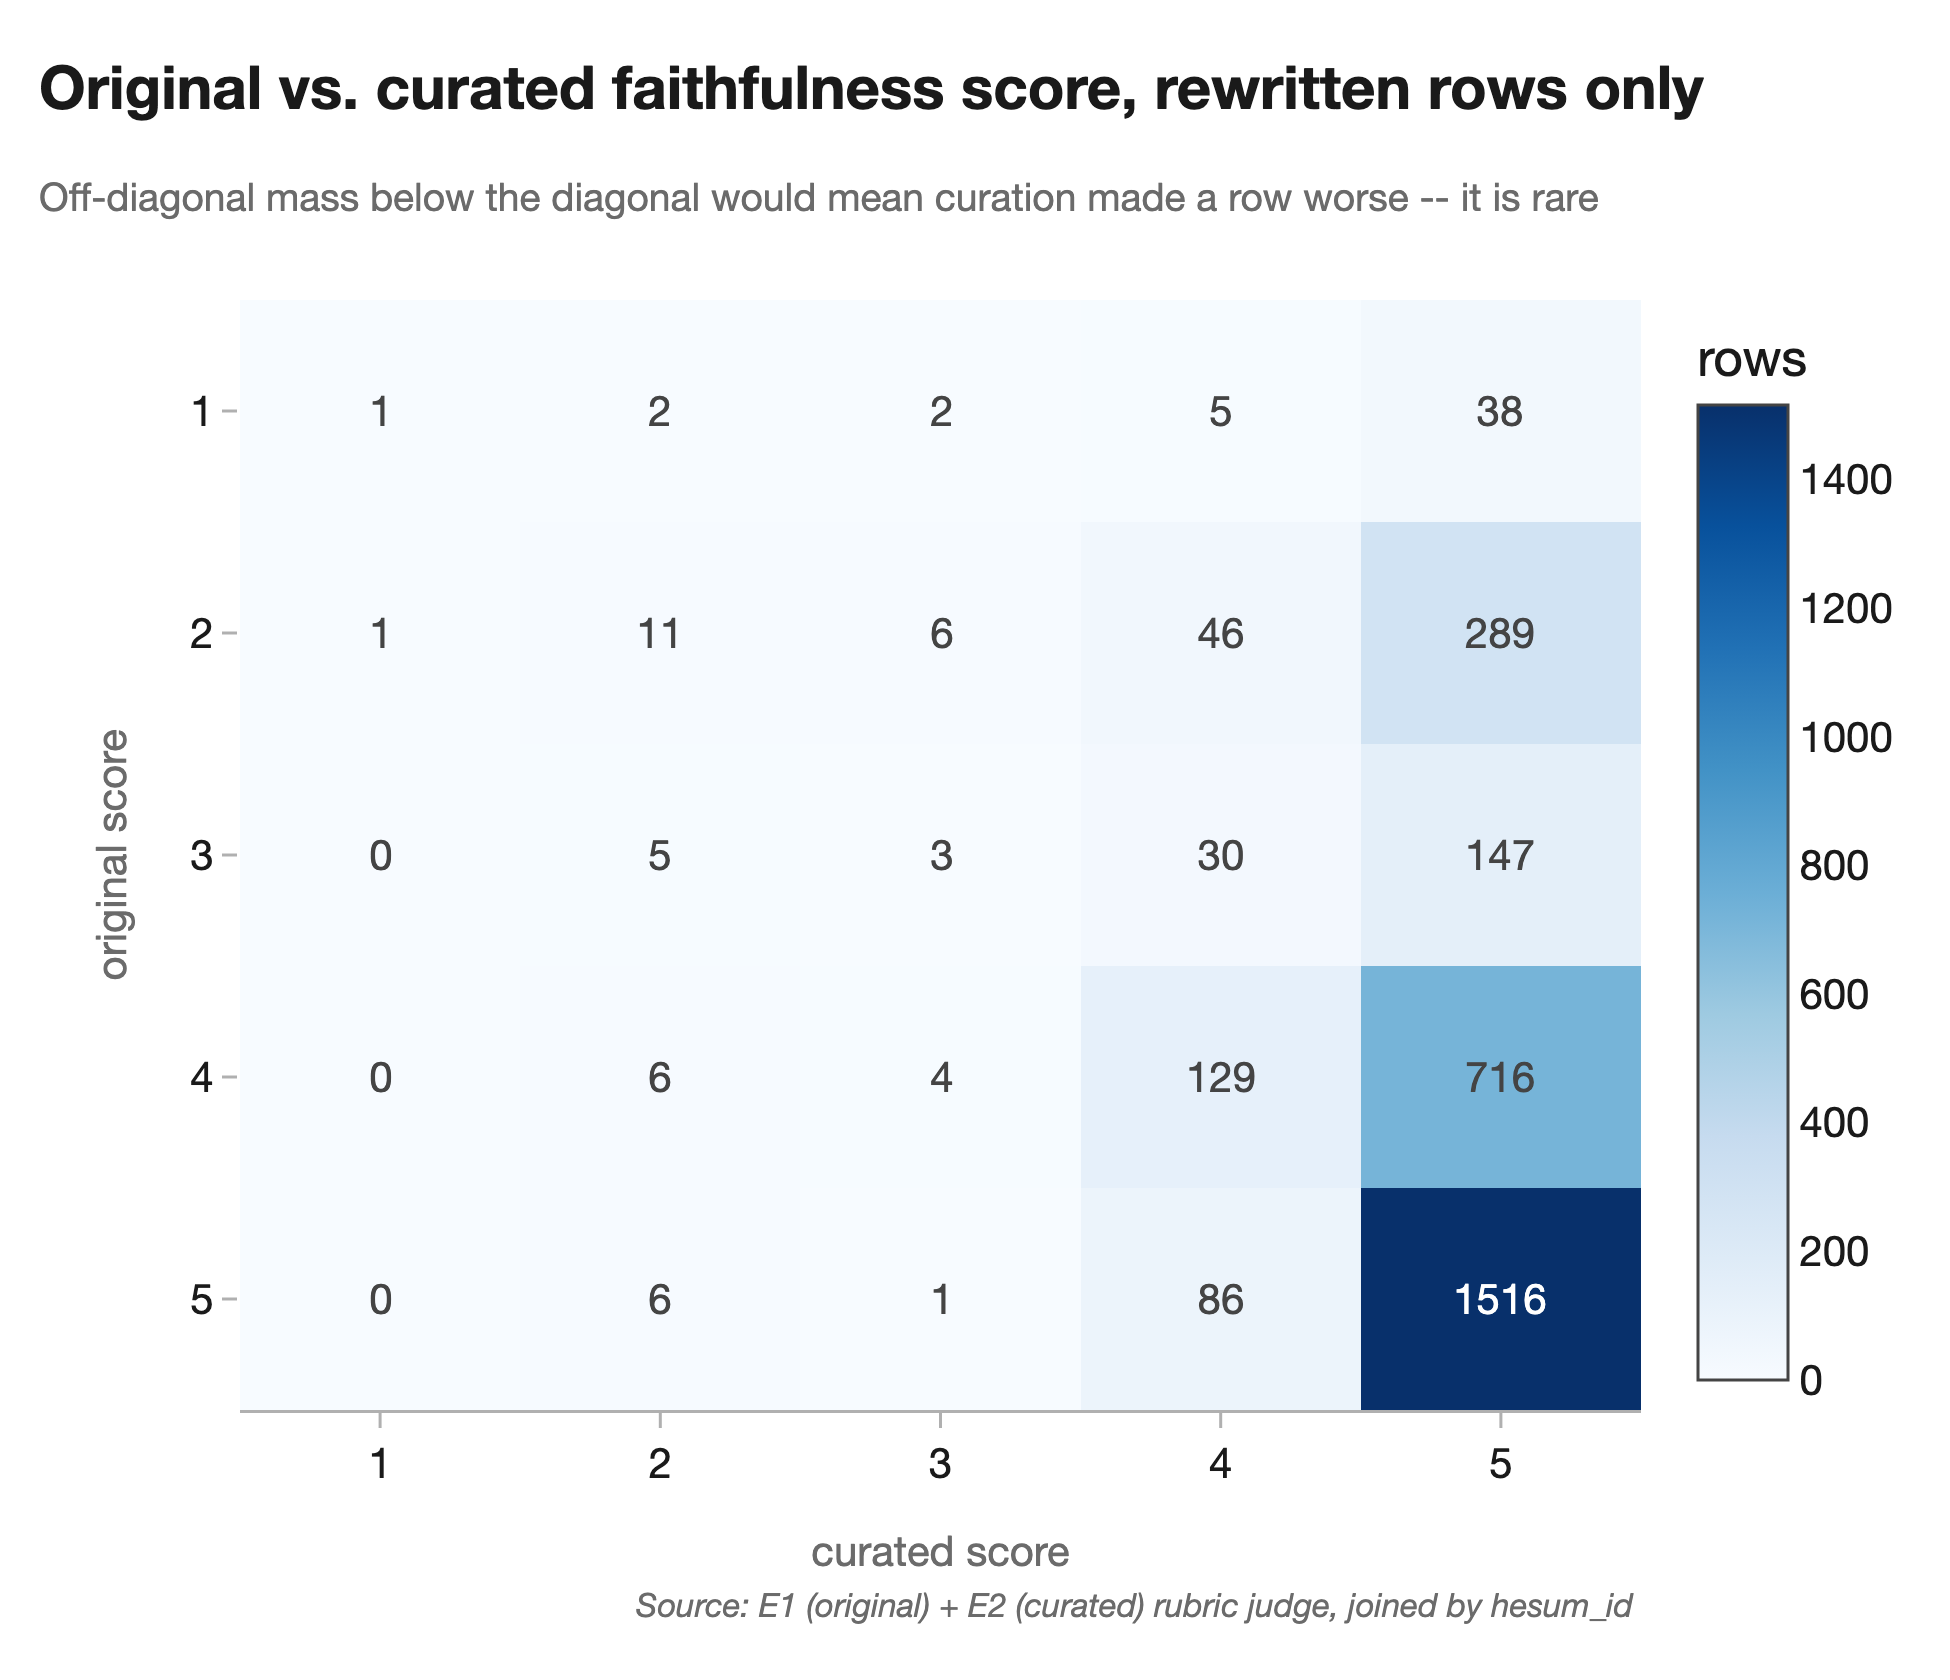
\includegraphics[width=\columnwidth]{figures/f6_transition_heatmap.png}
  \caption{Original vs.\ curated faithfulness score, rewritten rows only. Off-diagonal mass below the
  diagonal (curation making a row worse) is rare.}
  \label{fig:transition}
\end{figure}

\section{Interim fine-tuned vs.\ zero-shot comparison}
\label{app:finetuned-interim}
While Arm A training had not yet started at submission time (Section~\ref{sec:e4-results}), inference on
the partially-trained Arm B checkpoint reached $580$ of $586$ frozen-test-split predictions, enough for
an early look --against zero-shot \texttt{dicta-il/dictalm2.0-instruct} (the same base model as
Figure~\ref{fig:f9}), \emph{not} against Arm A. This is not the paper's E4 design: without Arm A, nothing
about curation follows from it (Section~\ref{sec:e4-methods}), and Arm B was fine-tuned for only $275$ of
$293$ steps before an infrastructure error interrupted it. We report it anyway as a caution sign.
Figure~\ref{fig:finetuned-interim} shows every headline edit sub-type and both stratified groups (S0
clean, S4 rewritten) scoring \emph{lower} for the fine-tuned checkpoint than for the zero-shot base model
on both LLM-judge dimensions, while ROUGE-1 and BERTScore are roughly tied (not shown). Two readings are
consistent with this: the checkpoint is under-trained ($94\%$ of one epoch, interrupted before
completion), or fine-tuning on this data degrades judged quality independent of which headline style it
targets. Distinguishing them requires the completed Arm A vs.\ Arm B comparison this appendix is a
placeholder for.

\begin{figure}[h]
  \centering
  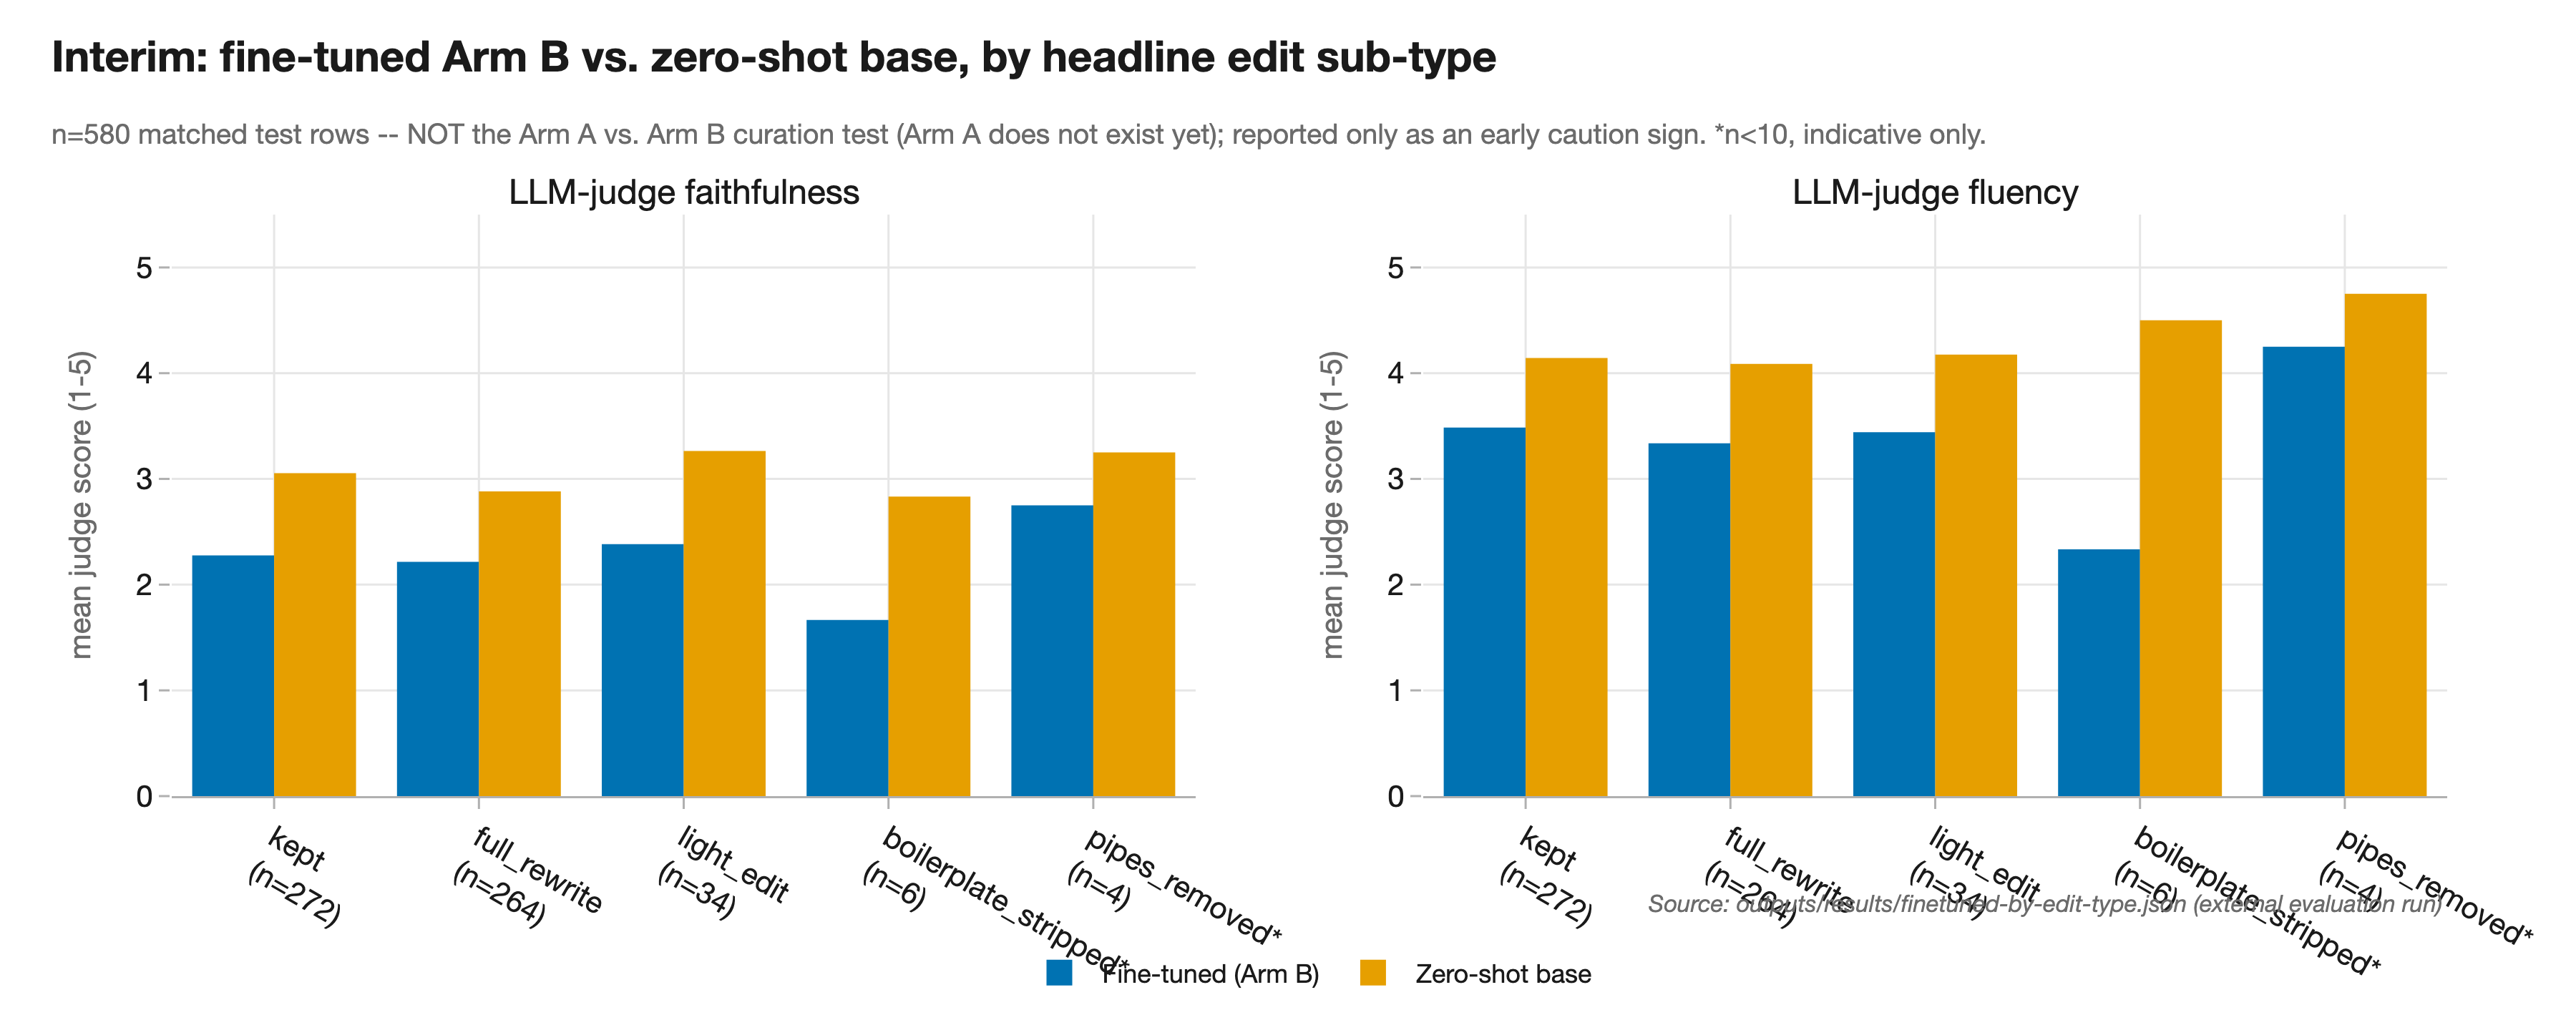
\includegraphics[width=\columnwidth]{figures/sx17_finetuned_vs_zeroshot.png}
  \caption{Interim: fine-tuned Arm B vs.\ zero-shot base by headline edit sub-type ($n=580$). Not the
  Arm A vs.\ Arm B curation test --reported as an early caution sign only.}
  \label{fig:finetuned-interim}
\end{figure}

\bibliography{bib}
\bibliographystyle{acl_natbib}

\end{document}
